%% ============================================================
%%  TFG — Inteligencia Artificial y Análisis Estadístico
%%       aplicado a la Industria Musical (Spotify)
%%  Autor: Roberto González Lozano
%%  Grado en Estadística — Universidad de Sevilla, 2026
%% ============================================================

\documentclass[12pt, a4paper, twoside]{book}

%% ── Codificación y fuentes ──────────────────────────────────
\usepackage[utf8]{inputenc}
\usepackage[T1]{fontenc}
\usepackage{lmodern}
\usepackage{microtype}

%% ── Idioma ──────────────────────────────────────────────────
\usepackage[spanish, es-tabla]{babel}

%% ── Márgenes ────────────────────────────────────────────────
\usepackage[top=3cm, bottom=3cm, left=3.5cm, right=2.5cm,
            headheight=15pt]{geometry}

%% ── Gráficos ────────────────────────────────────────────────
\usepackage{graphicx}
\graphicspath{{reports/figures/}}
\usepackage{float}
\usepackage{caption}
\usepackage{subcaption}

%% ── Tablas ──────────────────────────────────────────────────
\usepackage{booktabs}
\usepackage{multirow}
\usepackage{array}
\usepackage{longtable}
\usepackage{xcolor}
\usepackage{colortbl}

%% ── Matemáticas ─────────────────────────────────────────────
\usepackage{amsmath, amssymb, amsthm}

%% ── Código ──────────────────────────────────────────────────
\usepackage{listings}
\lstset{
  basicstyle=\small\ttfamily,
  breaklines=true,
  frame=single,
  backgroundcolor=\color{gray!10},
  keywordstyle=\color{blue!70}\bfseries,
  commentstyle=\color{green!50!black},
  stringstyle=\color{orange!80!black},
  numbers=left, numberstyle=\tiny\color{gray},
  language=Python
}

%% ── Cabeceras y pies ────────────────────────────────────────
\usepackage{fancyhdr}
\pagestyle{fancy}
\fancyhf{}
\fancyhead[LE]{\small\textit{\nouppercase{\leftmark}}}
\fancyhead[RO]{\small\textit{\nouppercase{\rightmark}}}
\fancyfoot[C]{\thepage}
\renewcommand{\headrulewidth}{0.4pt}

%% ── Hiperlinks ──────────────────────────────────────────────
\usepackage[colorlinks=true, linkcolor=blue!60!black,
            citecolor=green!50!black, urlcolor=blue!70]{hyperref}

%% ── Otros ───────────────────────────────────────────────────
\usepackage{setspace}
\usepackage{parskip}
\usepackage{enumitem}
\usepackage{csquotes}
\usepackage{lipsum}

%% ── Colores personalizados ──────────────────────────────────
\definecolor{verdeus}{rgb}{0.0, 0.50, 0.0}
\definecolor{azultfg}{rgb}{0.10, 0.25, 0.55}
\definecolor{gristabla}{rgb}{0.93, 0.93, 0.93}

%% ── Formato de capítulos ────────────────────────────────────
\usepackage{titlesec}
\titleformat{\chapter}[display]
  {\normalfont\huge\bfseries\color{azultfg}}
  {\chaptertitlename\ \thechapter}{18pt}{\Huge}
\titlespacing*{\chapter}{0pt}{0pt}{30pt}

%% ── Entornos de teoremas ─────────────────────────────────────
\theoremstyle{definition}
\newtheorem{definicion}{Definición}[chapter]
\newtheorem{observacion}{Observación}[chapter]

%% ============================================================
\begin{document}
\frontmatter

%% ── PORTADA ─────────────────────────────────────────────────
\begin{titlepage}
\centering
\vspace*{1.5cm}

{\large\bfseries UNIVERSIDAD DE SEVILLA}\\[0.3cm]
{\large Facultad de Matemáticas}\\[0.2cm]
{\large Grado en Estadística}\\[2cm]

\rule{\textwidth}{1.5pt}\\[0.5cm]
{\Huge\bfseries\color{azultfg}
Inteligencia Artificial y\\[0.3cm]
Análisis Estadístico\\[0.3cm]
aplicado a la\\[0.3cm]
Industria Musical}\\[0.4cm]
\rule{\textwidth}{1.5pt}\\[2cm]

{\Large\itshape Roberto González Lozano}\\[3cm]

\begin{minipage}{0.4\textwidth}
  \begin{flushleft}
    \emph{Tutor:}\\
    Dr.~[Nombre Tutor]
  \end{flushleft}
\end{minipage}
\hfill
\begin{minipage}{0.5\textwidth}
  \begin{flushright}
    Memoria presentada como parte\\
    de los requisitos para la obtención\\
    del título de Grado en Estadística\\
    por la Universidad de Sevilla
  \end{flushright}
\end{minipage}

\vfill
{\large Sevilla, Junio de 2026}
\end{titlepage}

\cleardoublepage

%% ── PÁGINA INTERIOR ─────────────────────────────────────────
\begin{center}
\vspace*{2cm}
{\Large\bfseries\color{azultfg}
Inteligencia Artificial y Análisis Estadístico\\
aplicado a la Industria Musical}\\[1.5cm]
{\large Roberto González Lozano}\\[1cm]
{\normalsize
Memoria presentada como parte de los requisitos\\
para la obtención del título de Grado en Estadística\\
por la Universidad de Sevilla.}\\[1.5cm]
Tutorizada por\\[0.3cm]
{\normalsize Dr.~[Nombre Tutor]}\\[0.3cm]
{\normalsize Dr.~[Nombre Cotutor (si procede)]}
\end{center}

\cleardoublepage

%% ── AGRADECIMIENTOS ─────────────────────────────────────────
\chapter*{Agradecimientos}
\addcontentsline{toc}{chapter}{Agradecimientos}

A mis padres y familia, por el apoyo incondicional durante estos años de carrera.

A mi tutor, por su guía y disposición a lo largo del desarrollo de este trabajo.

A Spotify, por poner a disposición de la comunidad investigadora conjuntos de
datos musicales que hacen posible trabajos como éste.

Y a la música, que es el objeto de estudio y también el acompañante de cada
jornada de trabajo.

\cleardoublepage

%% ── ABSTRACT (INGLÉS) ───────────────────────────────────────
\chapter*{English Abstract}
\addcontentsline{toc}{chapter}{English Abstract}

This Final Degree Project applies Artificial Intelligence and Statistical Analysis
techniques to the music industry, using a dataset of 114{,}000 tracks extracted
from Spotify with 21 variables per song, including audio features (danceability,
energy, valence, tempo, etc.) and the \texttt{popularity} index (0--100).

The work is structured in four methodological phases.
\textbf{Phase A} performs an exhaustive data audit: detection and imputation of
anomalous values, removal of extreme outliers in duration and loudness, and
feature engineering (log-transforms, popularity binary variable, electronic ratio
and a 12-category macro-genre map that reduces the original 114 genres to
interpretable groups).
\textbf{Phase B} carries out a deep Exploratory Data Analysis with ten analytical
axes: distribution of the target variable, Spearman correlations, violin plots by
macro-genre, scatter matrix, feature-vs-popularity relationships, genre radar charts,
confidence intervals for popularity, categorical variable effects, top artist analysis
and the specific study of songs with popularity = 0.
\textbf{Phase C} trains and compares two predictive ensemble models---Random
Forest and XGBoost---both for popularity regression and 12-class macro-genre
classification. Stratified train/test splitting, target encoding for the genre variable,
\texttt{RandomizedSearchCV} hyperparameter search, learning curve analysis and
SHAP explainability are included.
\textbf{Phase D} develops a music recommendation system based on three
strategies (global KNN, cluster-based and hybrid genre + KNN), evaluated through
proxy metrics without ground truth.

Key results: the popularity regression achieves $R^2 \approx 0.47$ (Random
Forest), confirming that audio features alone explain only a fraction of a song's
popularity; macro-genre classification reaches F1-macro $\approx 0.41$, well above
the 114-genre baseline; the optimal number of audio clusters is $k = 2$
(energetic vs.\ tranquil/acoustic), reflecting that Spotify's predefined features
capture an ``electronification'' dimension rather than fine stylistic nuances; and the
hybrid recommender achieves genre coherence = 1.0 with artist diversity = 0.83.

\cleardoublepage

%% ── RESUMEN ─────────────────────────────────────────────────
\chapter*{Resumen en español}
\addcontentsline{toc}{chapter}{Resumen en español}

El presente Trabajo de Fin de Grado aplica técnicas de Inteligencia Artificial y
Análisis Estadístico a la industria musical, empleando un conjunto de datos de
114.000 canciones extraído de Spotify con 21 variables por canción, entre las que
se encuentran \textit{audio features} (bailabilidad, energía, valencia, tempo, etc.)
y el índice de popularidad propio de la plataforma (escala 0--100).

El trabajo se articula en cuatro fases metodológicas de complejidad creciente.
La \textbf{Fase A} realiza una auditoría exhaustiva de calidad del dato: detección
e imputación de valores anómalos, eliminación de outliers extremos en duración y
loudness, y construcción de nuevas variables (transformaciones logarítmicas, variable
binaria de popularidad, ratio de electronización y mapa editorial de 12 macro-géneros
que reduce los 114 géneros originales a categorías interpretables).
La \textbf{Fase B} ejecuta un Análisis Exploratorio de Datos en profundidad con diez
ejes de análisis: distribución de la variable objetivo, correlaciones de Spearman,
violin plots por macro-género, scatter matrix entre audio features, relaciones
feature-vs-popularidad, radares de perfil sonoro por género, intervalos de confianza
para la popularidad media, efecto de variables categóricas, análisis de los artistas
más representados y estudio específico de canciones con popularidad cero.
La \textbf{Fase C} entrena y compara dos modelos predictivos de tipo \textit{ensemble}
---Random Forest y XGBoost--- tanto para regresión de popularidad como para
clasificación de macro-género en 12 clases. Se incluyen partición estratificada,
codificación de la variable género mediante \textit{target encoding}, búsqueda de
hiperparámetros con \texttt{RandomizedSearchCV}, curvas de aprendizaje y
explicabilidad mediante SHAP.
La \textbf{Fase D} desarrolla un sistema de recomendación musical basado en tres
estrategias (KNN global, basado en clúster e híbrido género + KNN), evaluadas
mediante métricas \textit{proxy} sin \textit{ground truth} real.

Los resultados clave son: la regresión de popularidad alcanza $R^2 \approx 0{,}47$
(Random Forest), confirmando que las audio features por sí solas explican solo
una fracción de la popularidad de una canción; la clasificación de macro-género
obtiene F1-macro $\approx 0{,}41$, muy por encima del \textit{baseline} con los
114 géneros sin agrupar; el número óptimo de clústeres de audio es $k = 2$
(energético vs.\ tranquilo/acústico), reflejando que las features predefinidas de
Spotify capturan una dimensión de ``electronización'' más que matices estilísticos
finos; y el recomendador híbrido alcanza coherencia de género = 1{,}0 con
diversidad de artistas = 0{,}83.

\cleardoublepage

%% ── ÍNDICE ──────────────────────────────────────────────────
\tableofcontents
\cleardoublepage
\listoffigures
\cleardoublepage
\listoftables
\cleardoublepage

%% ============================================================
\mainmatter
%% ============================================================

%% ── CAPÍTULO 1: INTRODUCCIÓN ────────────────────────────────
\chapter{Introducción}

\section{Motivación}

La industria musical genera anualmente miles de millones de euros y millones de
lanzamientos. Plataformas como Spotify concentran hoy más de 100 millones de
canciones y dan acceso a datos técnicos de audio sin precedentes. Este contexto abre
una oportunidad única para aplicar herramientas estadísticas y de Inteligencia
Artificial al estudio de la música: ¿qué hace a una canción popular? ¿Puede un
algoritmo aprender el ``sonido'' de un género a partir de sus características
físicas? ¿Es posible construir un sistema de recomendación basado únicamente en
datos cuantitativos de audio?

Estas preguntas motivan el presente Trabajo de Fin de Grado, que aborda un ciclo
completo de \textit{Data Science} aplicado a un dominio culturalmente relevante
y estadísticamente rico.

\section{El dataset de Spotify}

\subsection{Descripción general}

El dataset empleado contiene \textbf{114.000 registros} de canciones de Spotify
con 21 variables por registro. Fue publicado en Kaggle y corresponde a una
extracción de la API de Spotify realizada en 2022.

\begin{table}[H]
\centering
\caption{Variables del dataset de Spotify}
\label{tab:variables}
\begin{tabular}{lll}
\toprule
\textbf{Variable} & \textbf{Tipo} & \textbf{Descripción} \\
\midrule
\texttt{track\_id} & Cadena & Identificador único de la canción \\
\texttt{artists} & Cadena & Artista(s), separados por punto y coma \\
\texttt{album\_name} & Cadena & Nombre del álbum \\
\texttt{track\_name} & Cadena & Nombre de la canción \\
\texttt{popularity} & Entero [0-100] & Índice de popularidad de Spotify \\
\texttt{duration\_ms} & Entero & Duración en milisegundos \\
\texttt{explicit} & Booleano & Contenido explícito (sí/no) \\
\texttt{danceability} & Real [0-1] & Grado de bailabilidad \\
\texttt{energy} & Real [0-1] & Intensidad y actividad percibida \\
\texttt{key} & Entero [0-11] & Tonalidad musical \\
\texttt{loudness} & Real (dB) & Volumen medio en decibelios \\
\texttt{mode} & Binario & Modo Mayor (1) o Menor (0) \\
\texttt{speechiness} & Real [0-1] & Presencia de palabras habladas \\
\texttt{acousticness} & Real [0-1] & Grado de sonido acústico \\
\texttt{instrumentalness} & Real [0-1] & Ausencia de voz cantada \\
\texttt{liveness} & Real [0-1] & Probabilidad de actuación en directo \\
\texttt{valence} & Real [0-1] & Positividad musical percibida \\
\texttt{tempo} & Real (BPM) & Pulsaciones por minuto \\
\texttt{time\_signature} & Entero & Compás musical \\
\texttt{track\_genre} & Cadena & Género musical asignado \\
\bottomrule
\end{tabular}
\end{table}

\subsection{La variable \texttt{popularity}}

El índice de popularidad de Spotify es una \textbf{puntuación de 0 a 100}
calculada por un algoritmo propietario, basado principalmente en el volumen de
reproducciones recientes de la canción y su recencia. No representa el número
total de streams históricos ni el reconocimiento artístico global.

\begin{observacion}
La variable \texttt{popularity} debe entenderse como una \textbf{fotografía
instantánea} del momento en que se extrajo el dataset (2022). Una canción de 1965
con millones de reproducciones históricas puede tener \texttt{popularity} = 15 si
no tiene actividad reciente, mientras que una canción de 2022 recién lanzada puede
superar 80. Esta limitación es transversal a todo el análisis.
\end{observacion}

\subsection{Estructura de géneros}

El dataset original declara 125 géneros únicos, aunque tras la auditoría de datos
se verificaron \textbf{114 géneros reales}. La estructura es particular: Spotify
puede asignar una misma canción a varios géneros, por lo que el dataset contiene
una fila por combinación canción-género. Esto explica que, partiendo de 114.000
filas, solo existan \textbf{89.740 canciones únicas} por \texttt{track\_id}.

\section{Objetivos del trabajo}

El trabajo persigue cuatro objetivos principales, cada uno abordado en una fase:

\begin{enumerate}
  \item \textbf{Fase A — Limpieza exhaustiva}: construir un pipeline de
        preprocesado robusto y documentado que produzca un dataset de
        modelado de calidad, incluyendo ingeniería de variables.
  \item \textbf{Fase B — EDA profundo}: caracterizar estadísticamente el
        dataset mediante diez análisis gráficos y cuantitativos que sirvan de
        base para las decisiones de modelado.
  \item \textbf{Fase C — Modelos predictivos}: entrenar y comparar modelos
        Random Forest y XGBoost para la predicción de popularidad y la
        clasificación de macro-género, con búsqueda sistemática de
        hiperparámetros y análisis de explicabilidad SHAP.
  \item \textbf{Fase D — Clustering y recomendación}: agrupar canciones por
        similitud sonora y construir un sistema de recomendación musical
        \textit{content-based} evaluado con métricas proxy.
\end{enumerate}

\section{Estructura de la memoria}

Los capítulos 2, 3, 4 y 5 desarrollan respectivamente las cuatro fases descritas.
El capítulo 6 recoge las conclusiones globales y las líneas de trabajo futuro.
Los scripts Python generados están disponibles en el repositorio del proyecto.

%% ── CAPÍTULO 2: LIMPIEZA (FASE A) ──────────────────────────
\chapter{Limpieza Exhaustiva de Datos}

\section{Descripción del pipeline}

La limpieza de datos se realizó en varias etapas sucesivas y documentadas, con el
objetivo de producir un dataset de modelado (\texttt{tracks\_model.csv}) de
máxima calidad. La Tabla~\ref{tab:pipeline} resume el número de observaciones
en cada etapa.

\begin{table}[H]
\centering
\caption{Pipeline de limpieza: evolución del número de filas}
\label{tab:pipeline}
\rowcolors{2}{gristabla}{white}
\begin{tabular}{lrr}
\toprule
\textbf{Etapa} & \textbf{Filas} & \textbf{Cambio} \\
\midrule
Dataset original (\texttt{dataset.csv}) & 114.000 & --- \\
Tras eliminar fila nula & 113.999 & $-1$ \\
Tras deduplicación por \texttt{track\_id} & 89.740 & $-24.260$ \\
Tras excluir duración $< 0{,}5$ min o $> 15$ min & 89.585 & $-155$ \\
Tras excluir \texttt{loudness} $< -40$ dB & 89.550 & $-35$ \\
\textbf{Dataset de modelado final} & \textbf{89.550} & --- \\
\bottomrule
\end{tabular}
\end{table}

\section{Auditoría de calidad (Fase A.1)}

Antes de aplicar ninguna transformación, se ejecutó una auditoría completa de
calidad que comprueba los siguientes aspectos:

\begin{itemize}
  \item \textbf{Tipos de datos}: todas las variables numéricas tienen tipo correcto.
        La variable \texttt{explicit} es booleana y se convierte a entero (0/1)
        para el modelado.
  \item \textbf{Valores nulos}: una única fila con \texttt{artists},
        \texttt{album\_name} y \texttt{track\_name} nulos fue eliminada.
  \item \textbf{Unicidad de \texttt{track\_id}}: confirmada tras deduplicación.
  \item \textbf{Géneros con pocas canciones}: solo un género tiene menos de 100
        canciones, lo que asegura representatividad estadística.
\end{itemize}

La Tabla~\ref{tab:estadisticos} recoge las principales estadísticas descriptivas
de las variables numéricas en el dataset original.

\begin{table}[H]
\centering
\caption{Estadísticos descriptivos de las variables numéricas}
\label{tab:estadisticos}
\small
\rowcolors{2}{gristabla}{white}
\begin{tabular}{lrrrrrr}
\toprule
\textbf{Variable} & \textbf{Mín.} & \textbf{Máx.} & \textbf{Media} &
\textbf{Mediana} & \textbf{Desv.} & \textbf{Asim.} \\
\midrule
\texttt{popularity}       & 0     & 100   & 33,2  & 33    & 22,3  & 0,07  \\
\texttt{duration\_ms}     & 8.586 & 5.237.295 & 229.144 & 213.296 & 107.118 & 11,07 \\
\texttt{danceability}     & 0,00  & 0,99  & 0,562 & 0,576 & 0,176 & $-0,40$ \\
\texttt{energy}           & 0,00  & 1,00  & 0,634 & 0,676 & 0,258 & $-0,56$ \\
\texttt{loudness}         & $-49,5$ & 4,5 & $-8,5$ & $-7,2$ & 5,0  & $-1,96$ \\
\texttt{speechiness}      & 0,00  & 0,97  & 0,087 & 0,049 & 0,105 & 4,55  \\
\texttt{acousticness}     & 0,00  & 1,00  & 0,328 & 0,188 & 0,330 & 0,66  \\
\texttt{instrumentalness} & 0,00  & 1,00  & 0,173 & 0,000 & 0,315 & 1,56  \\
\texttt{liveness}         & 0,00  & 1,00  & 0,217 & 0,132 & 0,184 & 2,06  \\
\texttt{valence}          & 0,00  & 1,00  & 0,469 & 0,457 & 0,257 & 0,13  \\
\texttt{tempo}            & 30,2  & 243,4 & 122,2 & 122,0 & 29,7  & 0,29  \\
\bottomrule
\end{tabular}
\end{table}

\section{Tratamiento de outliers (Fase A.2)}

\subsection{Duración (\texttt{duration\_ms})}

Se convirtió la duración a minutos (\texttt{duration\_min}) para mayor
legibilidad. El análisis intercuartílico reveló:

$$Q_1 = 2{,}88 \text{ min}, \quad Q_3 = 4{,}40 \text{ min},
\quad \text{IQR} = 1{,}52 \text{ min}$$

Se identificaron \textbf{141 canciones de duración superior a 15 minutos}
(grabaciones de ambient, black metal o sesiones en directo) y \textbf{14 canciones
inferiores a 0{,}5 minutos} (intros, silencio o separadores). Ambos grupos fueron
excluidos del dataset de modelado por no representar canciones típicas.

\subsection{Loudness}

El rango habitual de \texttt{loudness} en audio digital es $[-30, 0]$ dB.
Se detectaron \textbf{35 filas con valores inferiores a $-40$ dB}, correspondientes
a grabaciones con problemas técnicos o silencio prácticamente total. Fueron excluidas.

\subsection{Tempo igual a cero}

En sesiones previas de limpieza (Fase 0) se detectaron 157 filas con
\texttt{tempo}$= 0$, que no representan canciones sin ritmo sino errores de
detección del algoritmo de Spotify. Fueron imputadas con la mediana del género
correspondiente:

$$\texttt{tempo}_i \leftarrow \operatorname{mediana}\{\texttt{tempo}_j : j
\in \text{mismo género que } i, \, \texttt{tempo}_j > 0\}$$

\subsection{Popularidad igual a cero}

El $10{,}5\%$ de las canciones (9.410 observaciones) presenta \texttt{popularity}$=0$.
Estas no son errores técnicos sino canciones con \textbf{muy pocas reproducciones
recientes} en el momento de la extracción. Se mantuvieron en el dataset porque
aportan información real sobre la distribución de popularidad.

\subsection{Hallazgo: canciones muy instrumentales y muy populares}

Se identificaron \textbf{194 canciones} con \texttt{instrumentalness}$> 0{,}9$ y
\texttt{popularity}$> 60$. Este grupo es una excepción interesante a la tendencia
general (correlación negativa entre ambas variables) y corresponde principalmente
a músicas de relajación o dormir (\textit{sleep sounds}), EDM instrumental y alguna
pieza de música clásica con alto número de reproducciones recientes.

\subsection{Correlaciones altas entre features de audio}

El análisis de correlación de Spearman entre variables predictoras reveló dos pares
con correlación $|r| > 0{,}70$:

\begin{table}[H]
\centering
\caption{Pares de features con posible multicolinealidad}
\label{tab:multicol}
\begin{tabular}{lc}
\toprule
\textbf{Par de variables} & $r_{\text{Spearman}}$ \\
\midrule
\texttt{energy} $\leftrightarrow$ \texttt{loudness}     & $+0{,}75$ \\
\texttt{energy} $\leftrightarrow$ \texttt{acousticness} & $-0{,}71$ \\
\bottomrule
\end{tabular}
\end{table}

Estas correlaciones implican redundancia de información. En modelos lineales
exigirían selección de variables o regularización. Sin embargo, los modelos de
\textit{ensemble} empleados en la Fase C (Random Forest y XGBoost) son
inherentemente robustos frente a la multicolinealidad, por lo que no se aplicó
ninguna eliminación.

\section{Ingeniería de variables (Fase A.3)}

A partir de las variables originales se construyeron las siguientes variables
derivadas:

\subsection{Transformaciones logarítmicas}

Tres variables presentan distribuciones muy sesgadas a la derecha con masa
concentrada cerca de cero: \texttt{instrumentalness}, \texttt{speechiness} y
\texttt{acousticness}. Para reducir el sesgo y mejorar la capacidad lineal de
los modelos se aplicó la transformación $\log(1+x)$:

\begin{align}
\texttt{log\_instrumentalness} &= \log(1 + \texttt{instrumentalness}) \\
\texttt{log\_speechiness} &= \log(1 + \texttt{speechiness}) \\
\texttt{log\_acousticness} &= \log(1 + \texttt{acousticness})
\end{align}

El uso de $\log(1+x)$ en lugar de $\log(x)$ evita problemas con valores iguales
a cero, que son frecuentes en estas variables.

\subsection{Variable binaria de popularidad}

Se creó la variable \texttt{is\_popular} $\in \{0, 1\}$ con umbral en 50:

$$\texttt{is\_popular} = \mathbf{1}[\texttt{popularity} \geq 50]$$

Con este umbral, el $23{,}7\%$ de las canciones se clasifica como popular. El valor 50
se eligió como punto de corte natural a la mitad de la escala y separa
aproximadamente el cuartil superior de la distribución.

\subsection{Ratio de electronización}

$$\texttt{electronic\_ratio} = \frac{\texttt{energy}}{\texttt{acousticness} + 0{,}01}$$

Este ratio actúa como \textit{proxy} de cuán electrónica (frente a acústica) es
una canción. El denominador incluye $0{,}01$ para evitar divisiones por cero.
Valores altos indican producciones muy electrónicas; valores bajos, música acústica.

\subsection{Mapa de macro-géneros}

Los 114 géneros originales del dataset se agruparon en \textbf{12 macro-categorías}
mediante un mapa editorial justificado en criterios musicológicos:

\begin{table}[H]
\centering
\caption{Distribución de canciones por macro-género tras el mapeo editorial}
\label{tab:macrogenre}
\rowcolors{2}{gristabla}{white}
\begin{tabular}{lrr}
\toprule
\textbf{Macro-género} & \textbf{Canciones} & \textbf{\%} \\
\midrule
Electrónica   & 15.635 & 17,5\% \\
World/Regional & 14.214 & 15,9\% \\
Pop           & 11.720 & 13,1\% \\
Rock          &  9.219 & 10,3\% \\
Metal         &  7.192 &  8,0\% \\
Folk/Acústico &  6.160 &  6,9\% \\
K-pop/J-pop   &  5.961 &  6,7\% \\
Otros (ambient, sleep, \ldots) &  5.813 &  6,5\% \\
Latino        &  4.156 &  4,6\% \\
Hip-hop/Trap  &  4.079 &  4,6\% \\
Jazz/Blues    &  2.913 &  3,3\% \\
Clásica       &  2.488 &  2,8\% \\
\bottomrule
\end{tabular}
\end{table}

La reducción de 114 a 12 categorías es esencial para la tarea de clasificación
de la Fase C: con 114 clases, muchas de ellas con apenas 1.000 observaciones y
fronteras estilísticas ambiguas, los clasificadores obtienen métricas muy bajas
que dificultan la interpretación. La agrupación en macro-géneros mejora
sustancialmente el F1-macro y produce resultados más interpretables.

%% ── CAPÍTULO 3: EDA PROFUNDO (FASE B) ──────────────────────
\chapter{Análisis Exploratorio de Datos}

\section{Introducción al EDA}

El Análisis Exploratorio de Datos (EDA) es la etapa previa a cualquier modelado
y tiene como objetivo comprender la estructura de los datos, detectar anomalías,
estudiar las relaciones entre variables y formular hipótesis. En este trabajo el
EDA se articula en \textbf{diez análisis} complementarios que cubren la variable
objetivo, las relaciones entre predictores, los perfiles sonoros por género y el
comportamiento de subpoblaciones específicas.

Todos los análisis se realizaron sobre \texttt{tracks\_model.csv} (89.550
canciones, 29 variables) mediante Python con las bibliotecas \texttt{pandas},
\texttt{numpy}, \texttt{matplotlib}, \texttt{seaborn} y \texttt{scipy.stats}.

\section{Distribución de la variable objetivo (B.1)}

La Figura~\ref{fig:B1} muestra tres representaciones complementarias de la
distribución de \texttt{popularity}: histograma con estimación de densidad kernel,
diagrama de caja y función de distribución empírica acumulada (ECDF).

\begin{figure}[H]
  \centering
  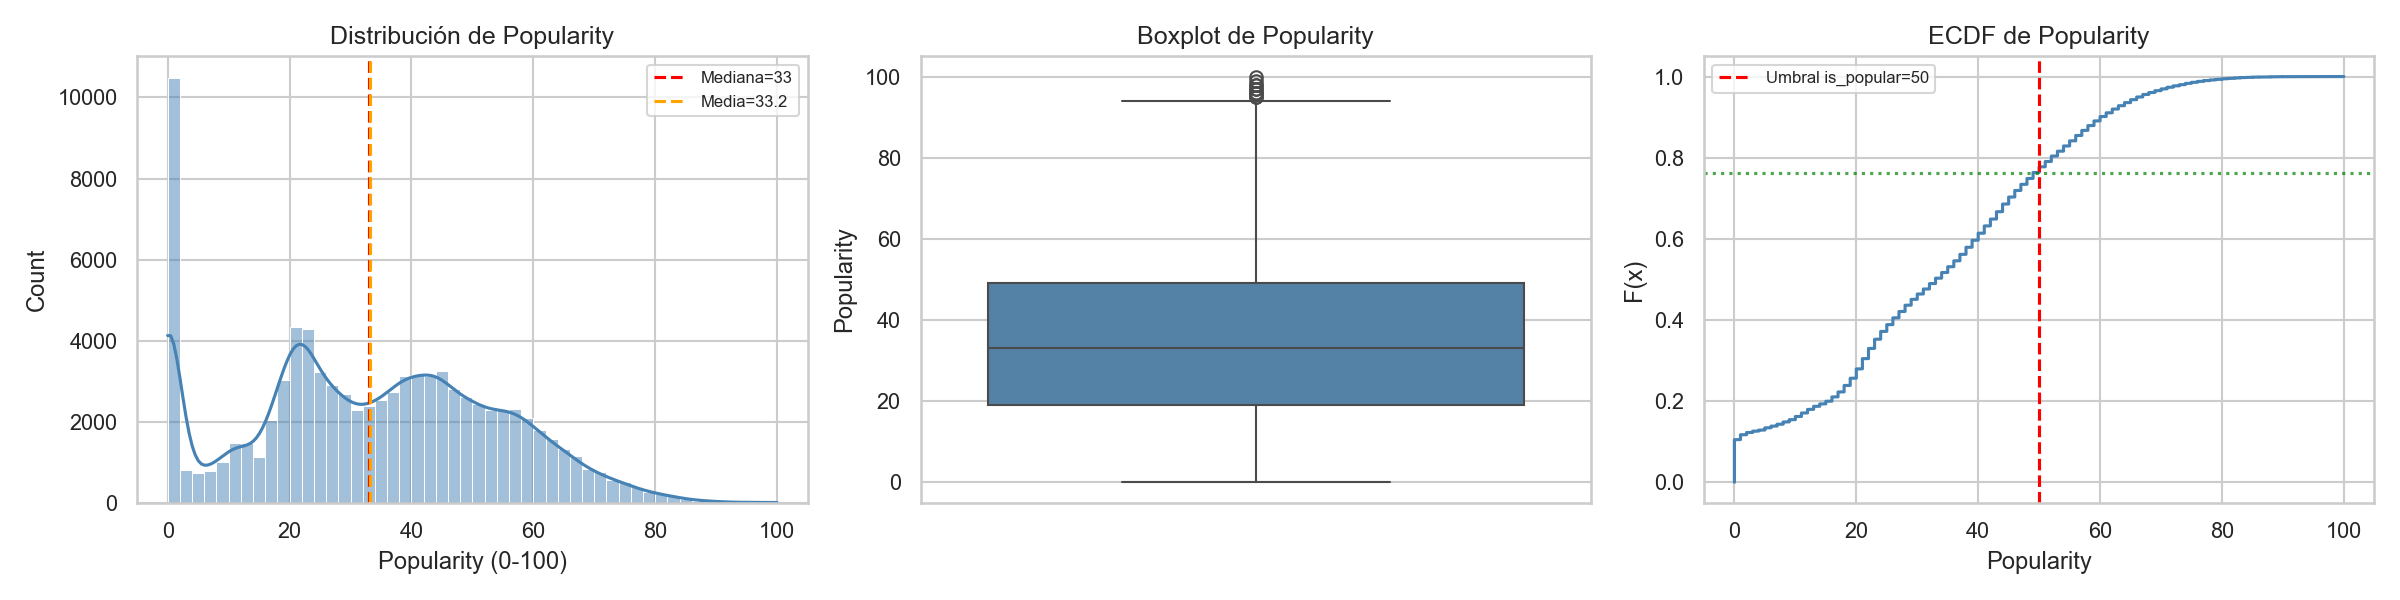
\includegraphics[width=\textwidth]{B1_popularity_distribution}
  \caption{Distribución de la variable \texttt{popularity}.
           Izquierda: histograma con KDE. Centro: boxplot.
           Derecha: ECDF con umbral \texttt{is\_popular} = 50.}
  \label{fig:B1}
\end{figure}

Los tests formales de normalidad confirman el alejamiento de la distribución
gaussiana:

\begin{itemize}
  \item \textbf{Shapiro-Wilk} (sobre muestra $n=5.000$):
        $W = 0{,}9706$, $p < 10^{-30}$ $\Rightarrow$ se rechaza la normalidad.
  \item \textbf{Kolmogorov-Smirnov} (contra normal estándar tras estandarización):
        $D = 0{,}0589$, $p < 10^{-15}$ $\Rightarrow$ se rechaza la normalidad.
\end{itemize}

La distribución presenta un sesgo de $0{,}07$ (prácticamente simétrico en su
parte central) pero con un pico marcado en $\texttt{popularity} = 0$ que
representa el $10{,}5\%$ de las observaciones. Este comportamiento bimodal
anticipa la dificultad del problema de regresión: el modelo ha de aprender a
predecir tanto el pico en cero como la distribución continua del cuerpo principal.

\section{Correlaciones de Spearman con la popularidad (B.2)}

Se calculó el coeficiente de correlación de Spearman entre cada predictor numérico
y la variable \texttt{popularity}. Se eligió Spearman (en lugar de Pearson) por
su robustez frente a distribuciones no normales y relaciones monótonas no lineales.
La Figura~\ref{fig:B2} muestra los resultados.

\begin{figure}[H]
  \centering
  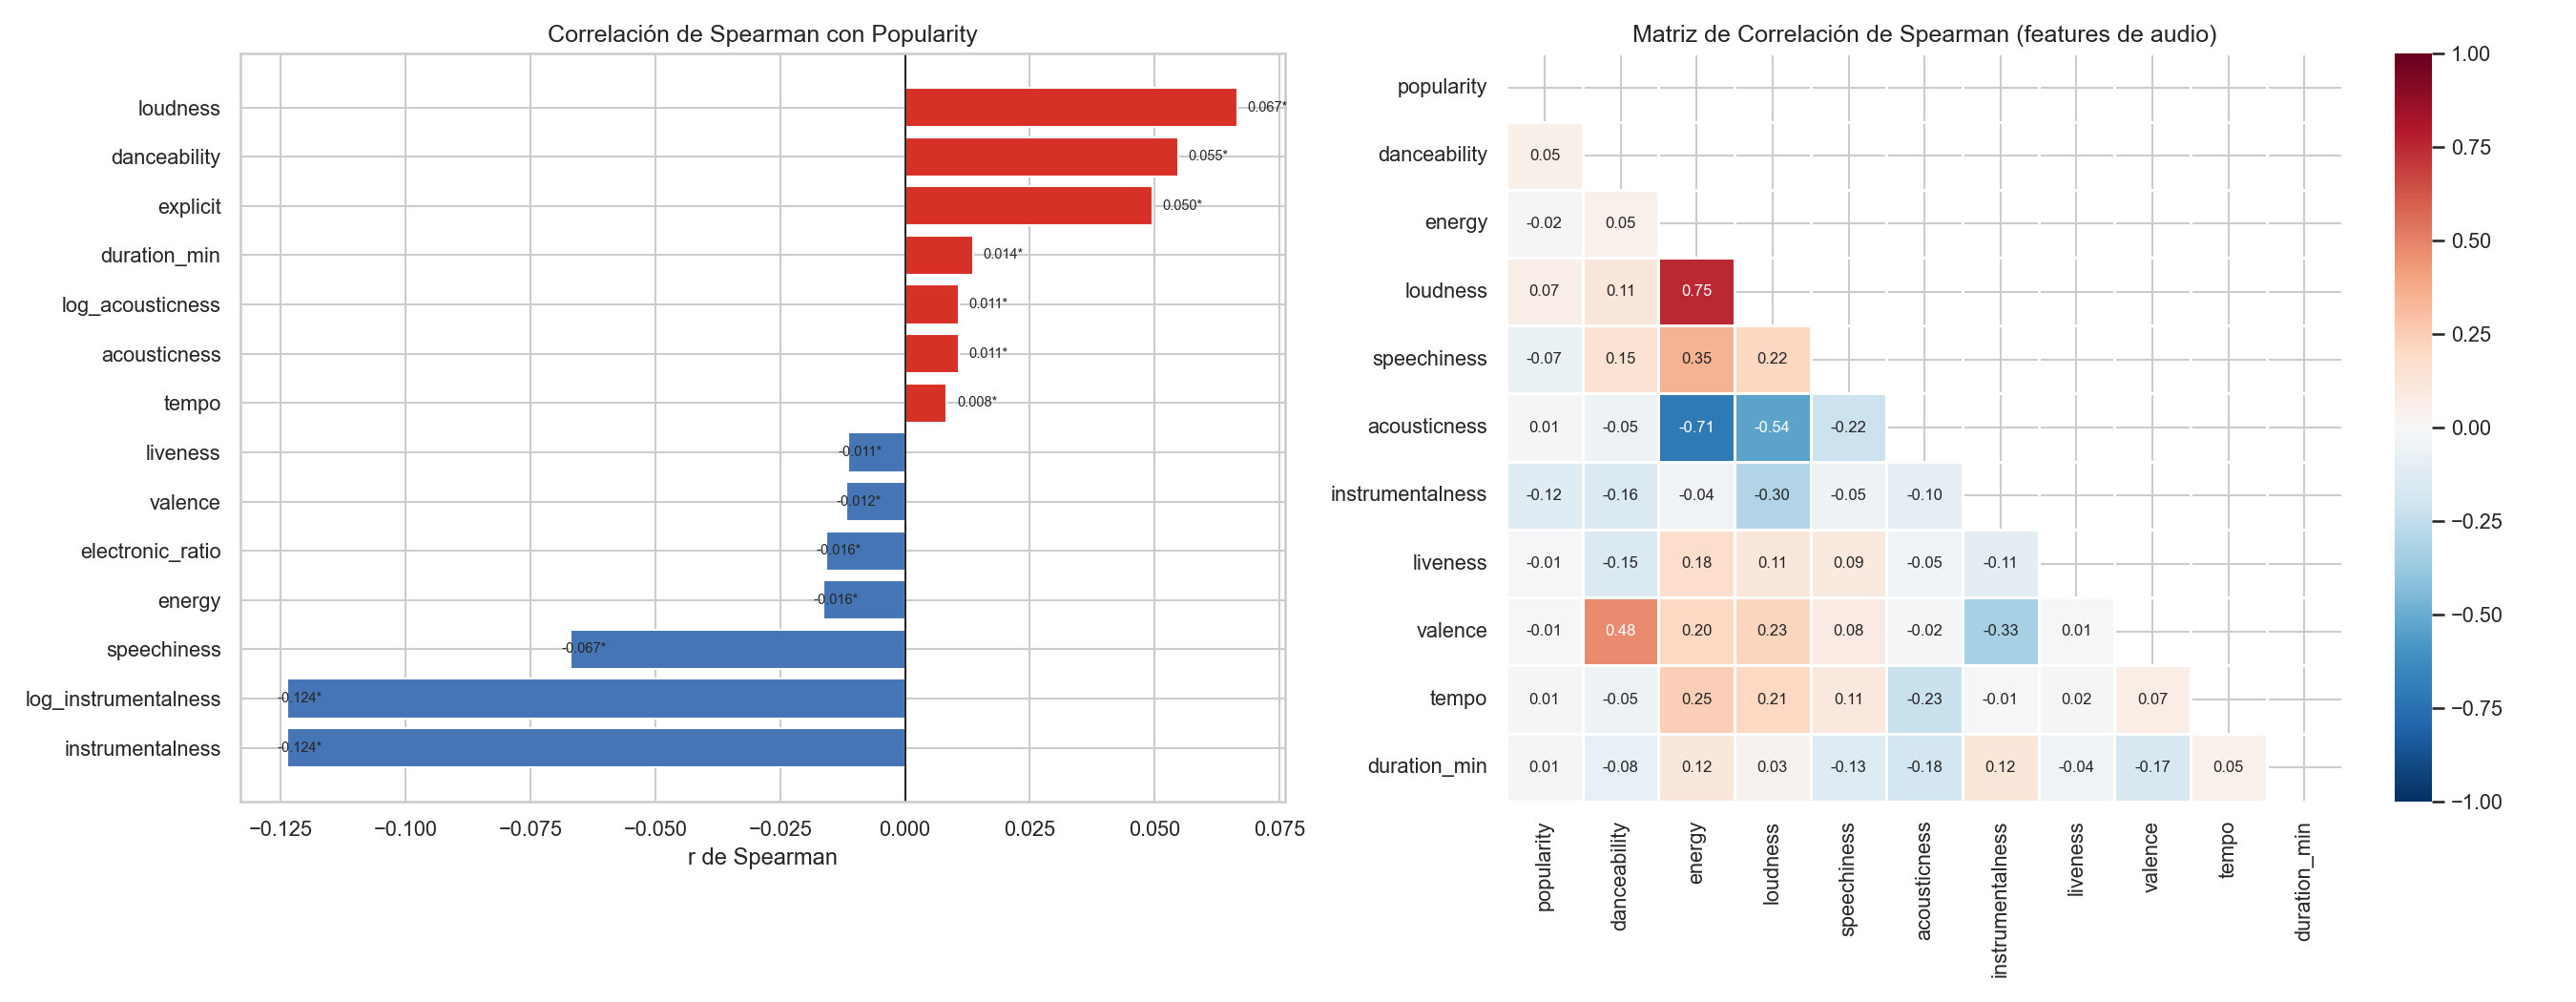
\includegraphics[width=\textwidth]{B2_correlation_heatmap}
  \caption{Izquierda: correlaciones de Spearman de cada feature con
           \texttt{popularity} (barras rojas = positiva, azules = negativa).
           Derecha: matriz de correlación de Spearman entre features de audio
           (solo triángulo inferior).}
  \label{fig:B2}
\end{figure}

\begin{table}[H]
\centering
\caption{Correlaciones de Spearman con \texttt{popularity} (selección)}
\label{tab:corr_pop}
\rowcolors{2}{gristabla}{white}
\begin{tabular}{lcc}
\toprule
\textbf{Feature} & $r_{\text{Spearman}}$ & \textbf{$p$-valor} \\
\midrule
\texttt{instrumentalness}     & $-0{,}124$ & $< 10^{-300}$ \\
\texttt{log\_instrumentalness}& $-0{,}124$ & $< 10^{-300}$ \\
\texttt{speechiness}          & $-0{,}067$ & $< 10^{-88}$  \\
\texttt{energy}               & $-0{,}016$ & $< 0{,}001$   \\
\texttt{tempo}                & $+0{,}008$ & $0{,}012$     \\
\texttt{danceability}         & $+0{,}055$ & $< 10^{-60}$  \\
\texttt{loudness}             & $+0{,}067$ & $< 10^{-88}$  \\
\texttt{explicit}             & $+0{,}050$ & $< 10^{-49}$  \\
\bottomrule
\end{tabular}
\end{table}

Dos conclusiones destacan:

\begin{enumerate}
  \item Todas las correlaciones son estadísticamente significativas (muestras
        grandes con $n \approx 90.000$), pero su magnitud es muy baja
        ($|r| < 0{,}13$). Esto confirma que ninguna feature de audio individual
        tiene poder predictivo suficiente por sí sola.
  \item La correlación negativa más fuerte la tiene \texttt{instrumentalness}:
        las canciones sin voz cantada tienden a ser menos populares en el
        snapshot de Spotify. Esto refleja un sesgo del índice hacia géneros
        vocales urbanos (pop, hip-hop, reggaeton) en el período analizado.
\end{enumerate}

\section{Violin plots por macro-género (B.3)}

La Figura~\ref{fig:B3} compara la distribución de seis audio features entre los
doce macro-géneros mediante violin plots, que combinan la información del boxplot
(mediana, cuartiles) con la densidad de probabilidad estimada por KDE.

\begin{figure}[H]
  \centering
  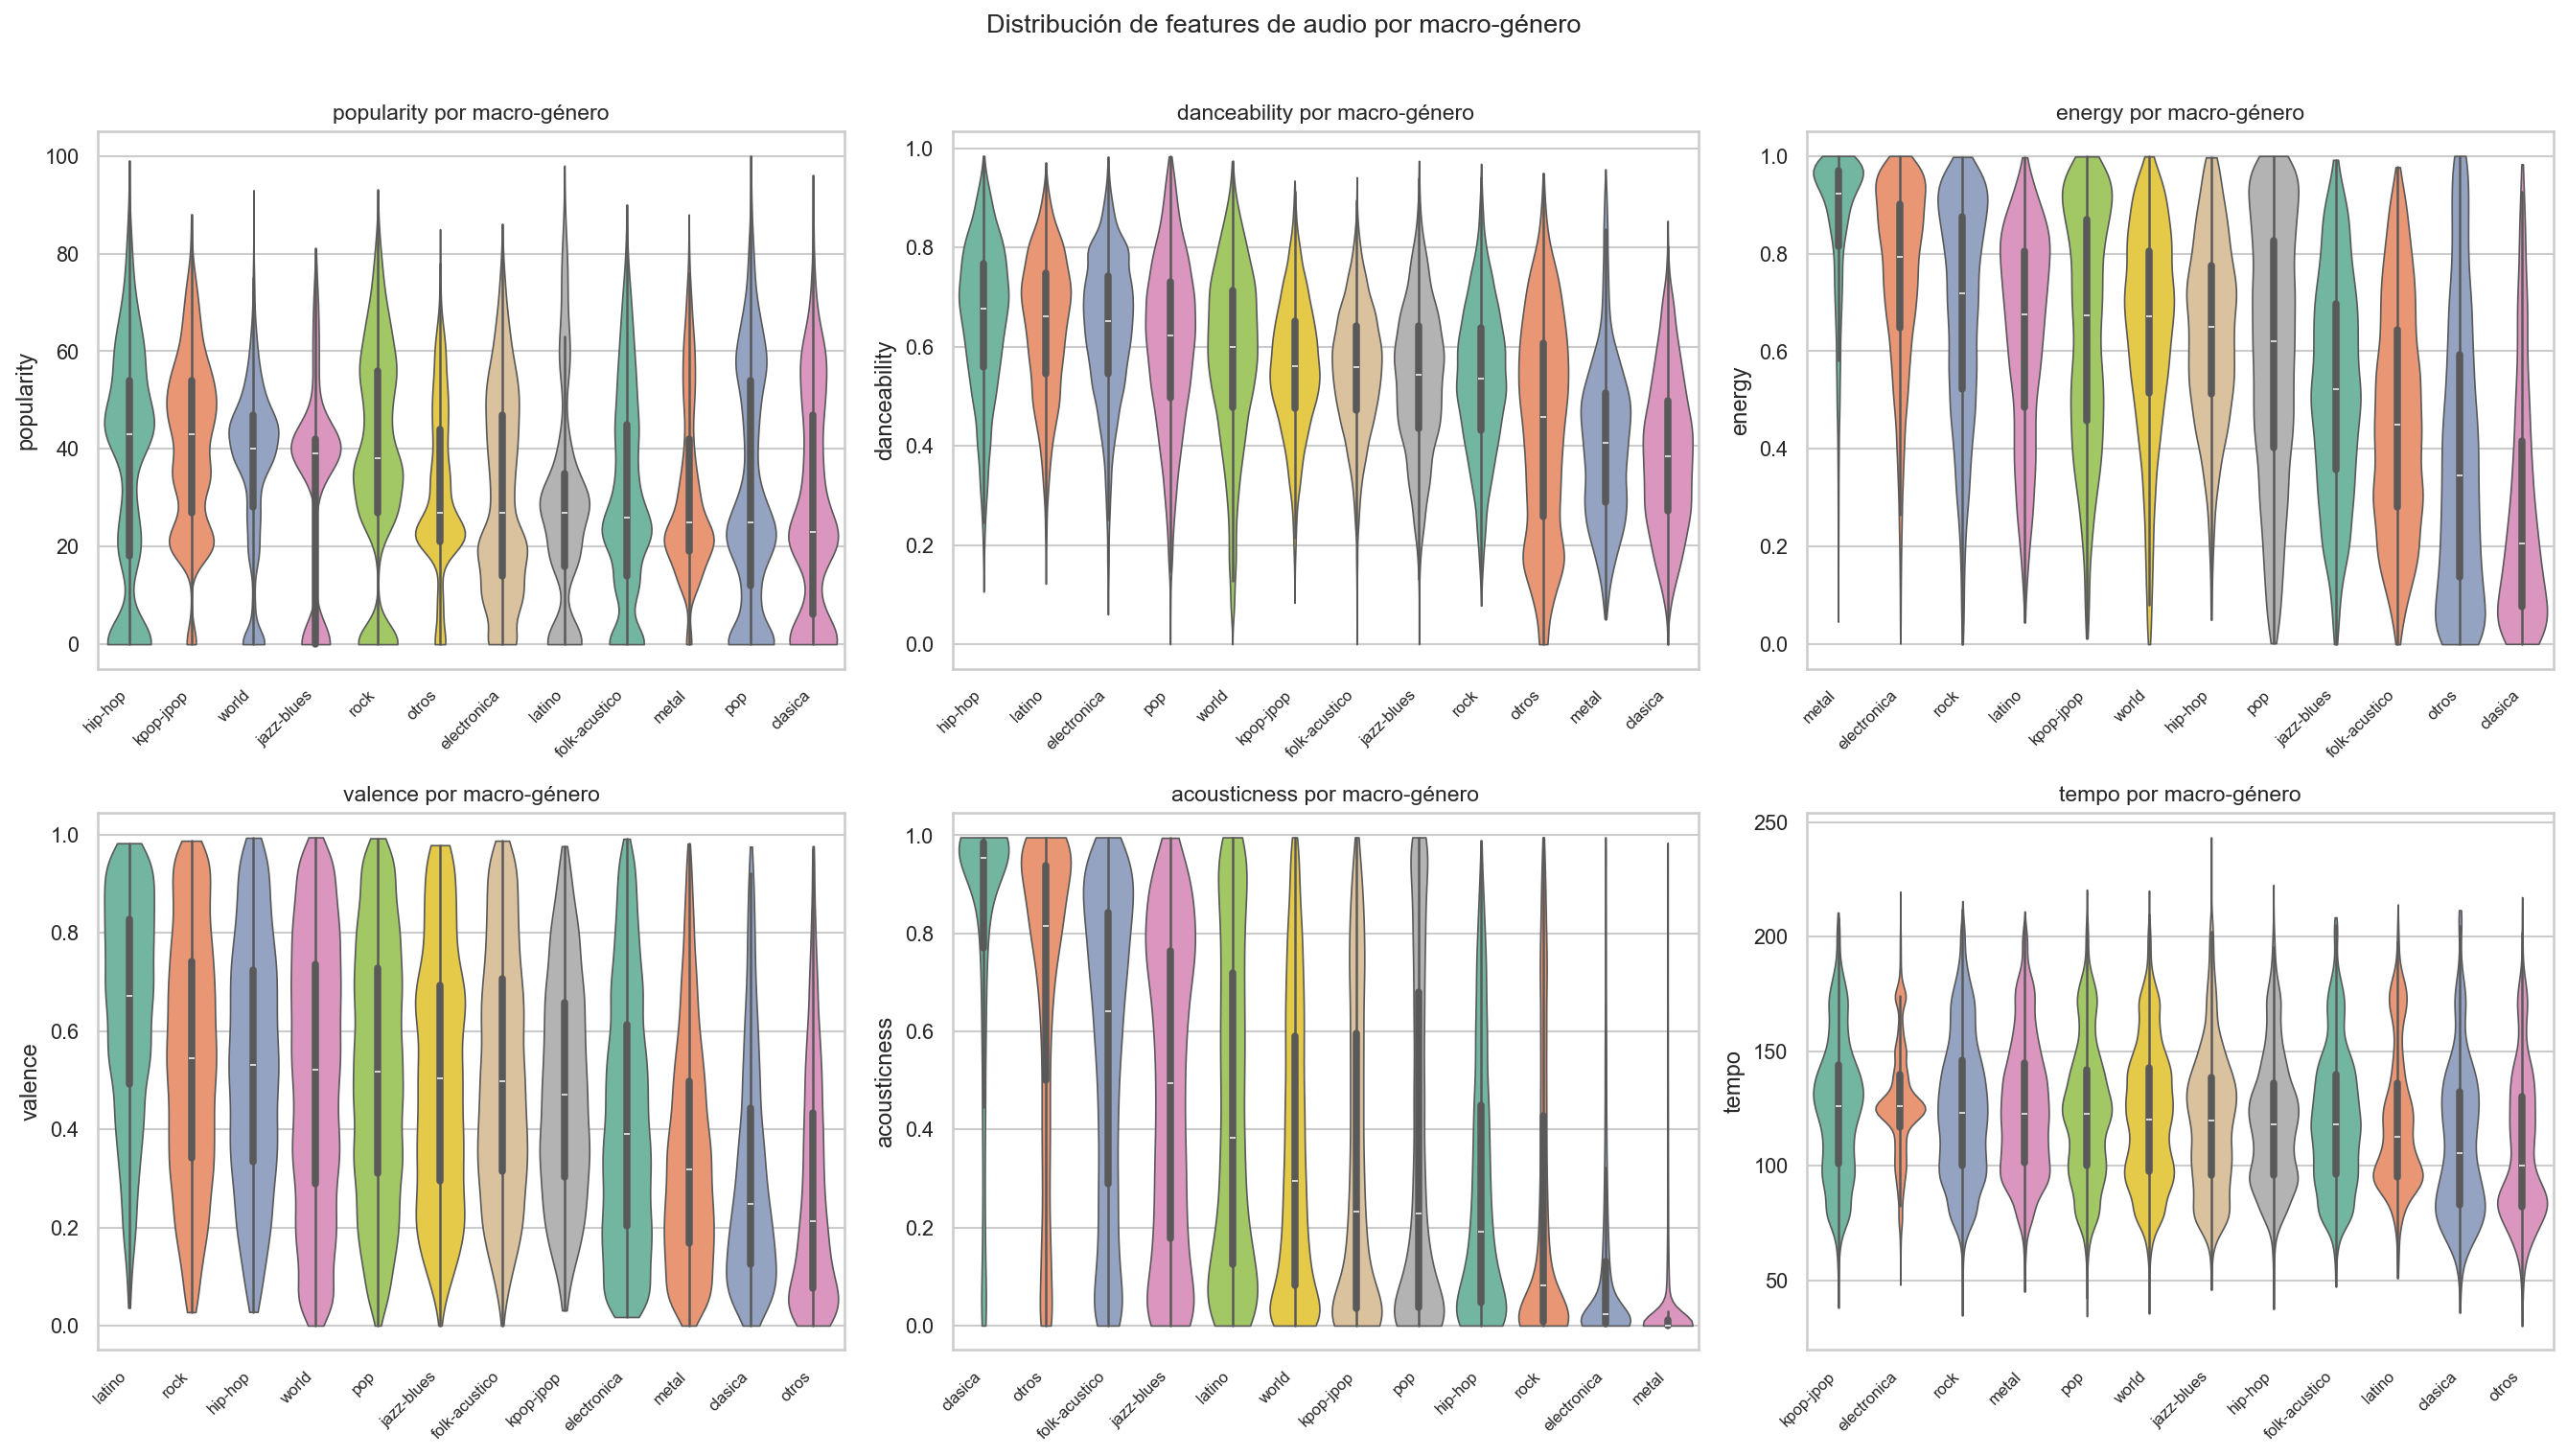
\includegraphics[width=\textwidth]{B3_violin_by_macrogenre}
  \caption{Distribución de seis audio features por macro-género (violin plots).
           Los géneros están ordenados por mediana decreciente en cada panel.}
  \label{fig:B3}
\end{figure}

Los hallazgos más relevantes son:

\begin{itemize}
  \item En \textbf{popularidad}, hip-hop encabeza la clasificación (mediana = 43)
        seguido de pop y kpop-jpop. La música clásica presenta la mediana más
        baja (23), fundamentalmente por el efecto de recencia del índice.
  \item En \textbf{danceability}, los géneros latinos y el kpop concentran
        sus distribuciones por encima de $0{,}70$, mientras que la música
        clásica y el metal presentan medianas por debajo de $0{,}50$.
  \item En \textbf{energy}, el metal destaca con una distribución muy
        concentrada en valores altos ($> 0{,}85$). La clásica y el folk-acústico
        tienen las medianas más bajas.
  \item Varios géneros presentan distribuciones bimodales (especialmente en
        acousticness), lo que sugiere la existencia de subpoblaciones con
        características sonoras muy distintas dentro de una misma macro-categoría.
\end{itemize}

\section{Scatter matrix de audio features (B.4)}

La Figura~\ref{fig:B4} muestra una matriz de dispersión entre seis audio
features clave, coloreada por macro-género sobre una muestra de 4.000 canciones.

\begin{figure}[H]
  \centering
  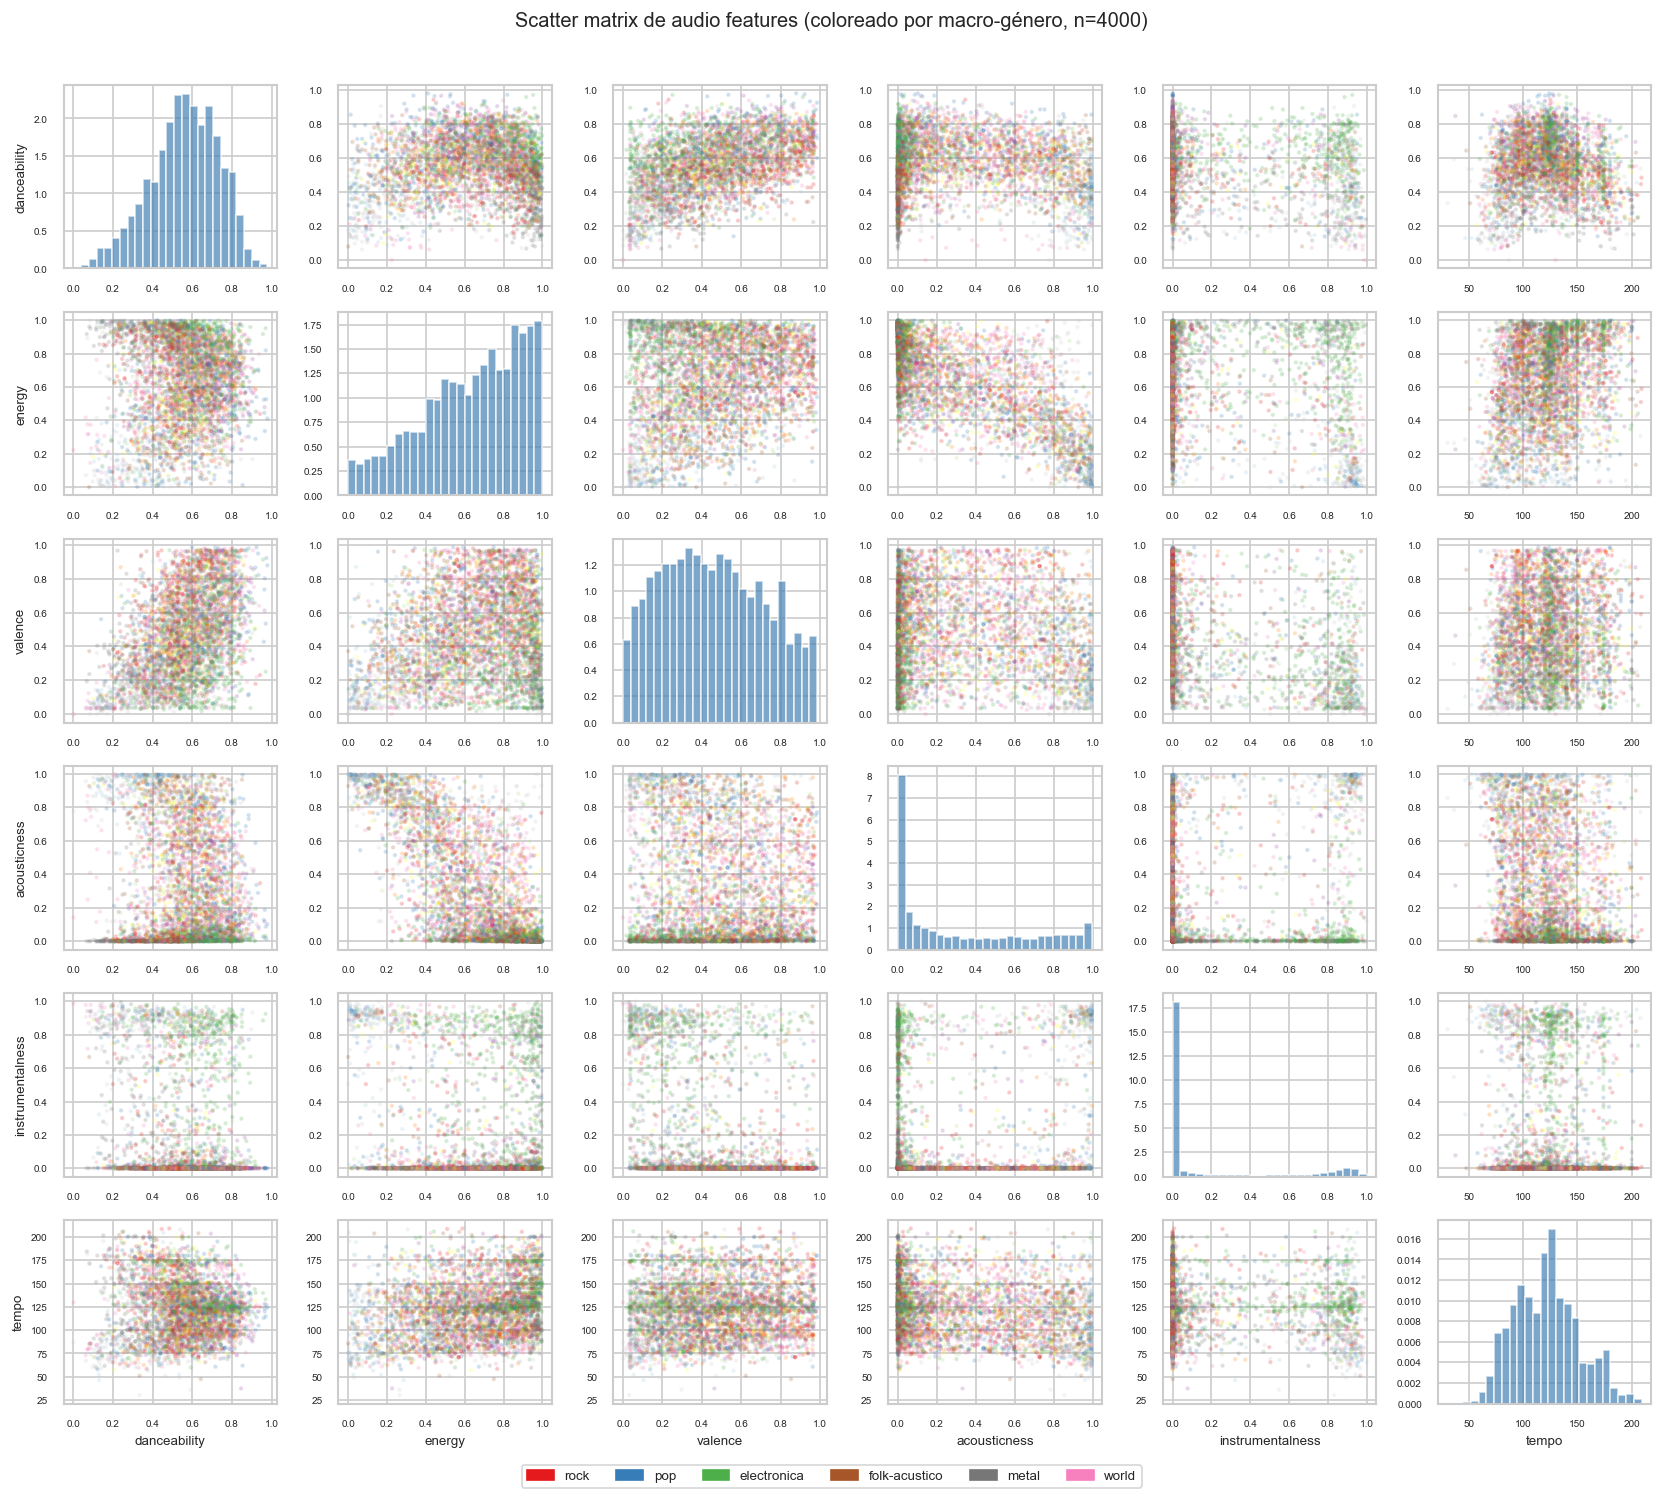
\includegraphics[width=\textwidth]{B4_scatter_matrix}
  \caption{Scatter matrix entre danceability, energy, valence, acousticness,
           instrumentalness y tempo. Coloreado por macro-género (n = 4.000).}
  \label{fig:B4}
\end{figure}

La pareja \textbf{energy--acousticness} es la más informativa: presenta una
correlación negativa clara ($r_S = -0{,}71$) y permite distinguir visualmente
dos grandes nubes de puntos: música electrónica/metal (alta energy, baja
acousticness) y música clásica/folk-acústico (baja energy, alta acousticness).
Esta estructura es coherente con que el clustering de la Fase D converja
a $k = 2$ clústeres: el espacio de audio features tiene una dimensión dominante
de ``electronización vs. acústica''.

La variable \texttt{instrumentalness} es llamativamente bimodal en su distribución
marginal: la gran mayoría de canciones tiene valores cercanos a cero (canciones
con voz), mientras que un segundo grupo con valores $> 0{,}8$ corresponde a
música clásica, ambient y EDM instrumental.

\section{Features vs. Popularidad (B.5)}

La Figura~\ref{fig:B5} muestra scatter plots de cada feature contra
\texttt{popularity} (muestra de 6.000 canciones) con línea de tendencia lineal.

\begin{figure}[H]
  \centering
  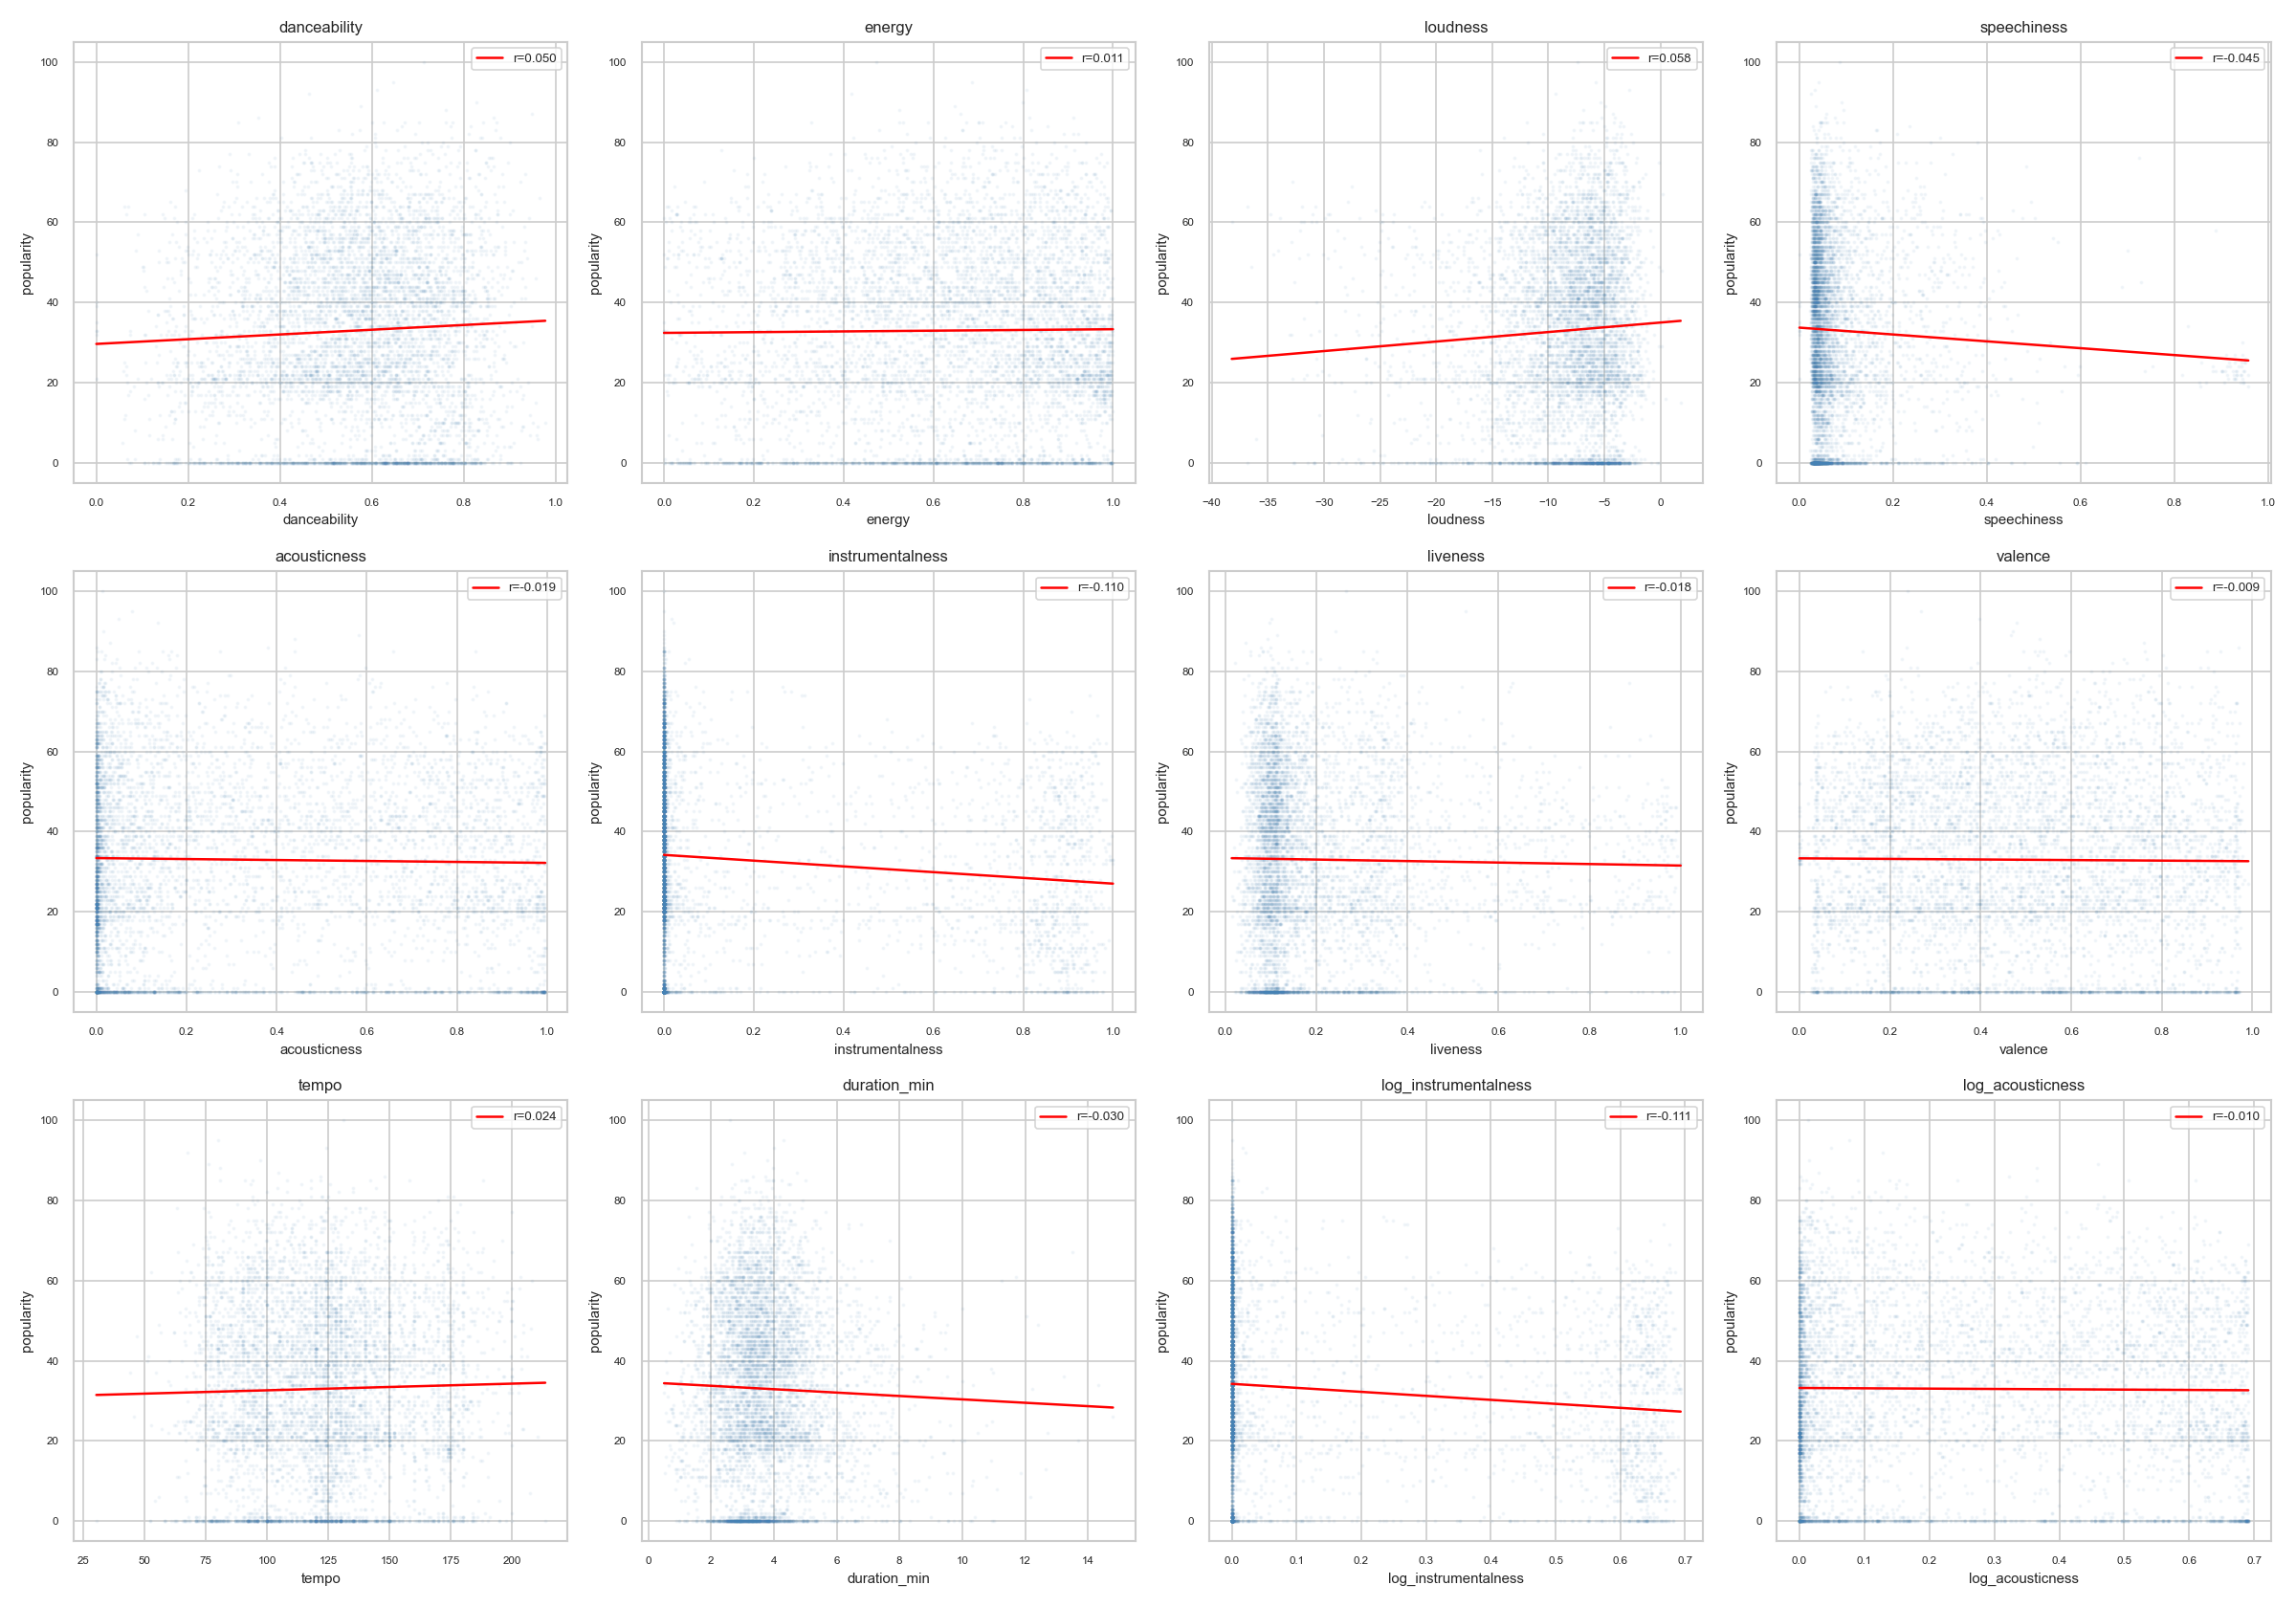
\includegraphics[width=\textwidth]{B5_features_vs_popularity}
  \caption{Relación entre cada audio feature (y sus log-transformadas) con
           \texttt{popularity}. La línea roja es la regresión lineal simple.
           El coeficiente de Pearson $r$ se indica en la leyenda de cada panel.}
  \label{fig:B5}
\end{figure}

El ruido extremo en todos los paneles confirma la dificultad del problema:
la nube de puntos es prácticamente uniforme para cualquier valor de las
features. Las transformaciones logarítmicas de \texttt{instrumentalness} y
\texttt{acousticness} producen relaciones lineales ligeramente más pronunciadas,
justificando su inclusión como variables adicionales en los modelos de la Fase C.

\section{Perfil sonoro por macro-género: gráfico radar (B.6)}

El gráfico radar de la Figura~\ref{fig:B6} representa el perfil medio de siete
audio features (normalizadas a $[0,1]$) para diez macro-géneros simultáneamente,
permitiendo comparar su ``sonido característico'' de forma visual e intuitiva.

\begin{figure}[H]
  \centering
  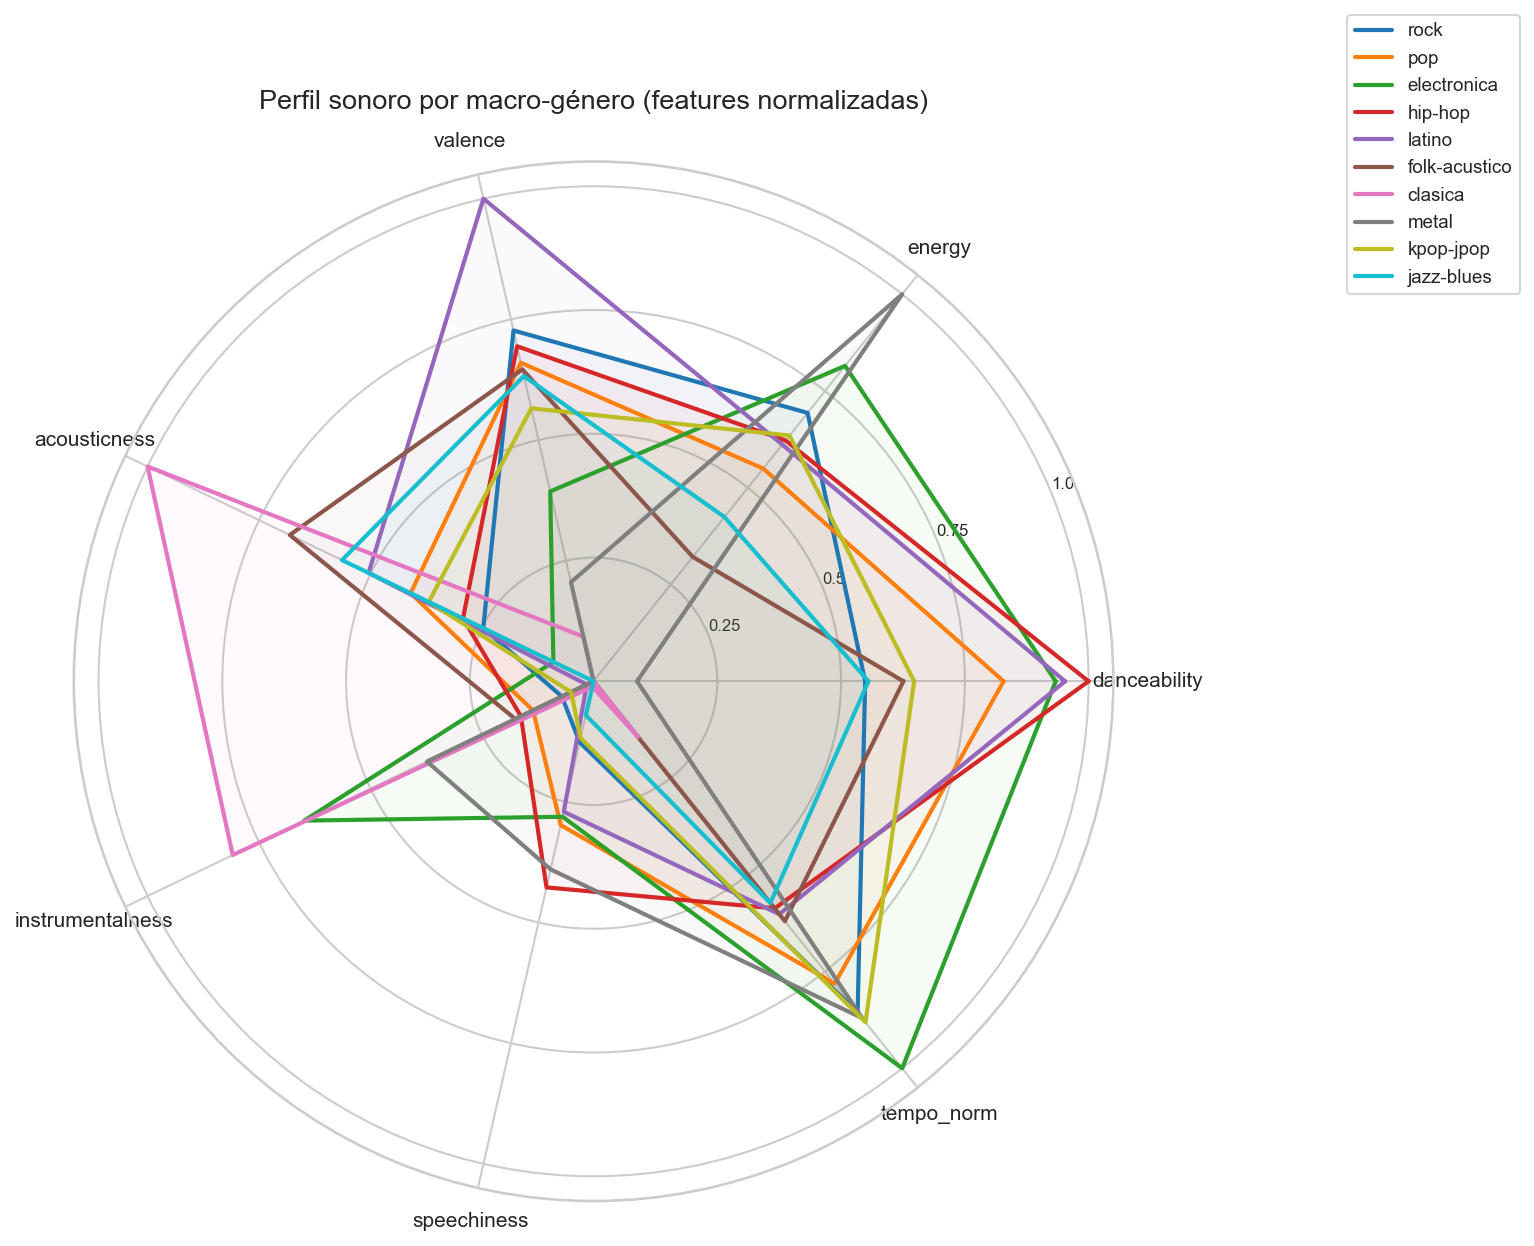
\includegraphics[width=0.85\textwidth]{B6_radar_by_macrogenre}
  \caption{Gráfico radar del perfil sonoro medio por macro-género.
           Cada eje representa una audio feature normalizada a [0,1].}
  \label{fig:B6}
\end{figure}

Las diferencias entre géneros son notables y musicalmente coherentes:

\begin{itemize}
  \item \textbf{Metal}: energy extrema, valence mínima (sonido intenso y oscuro),
        acousticness nula.
  \item \textbf{Clásica}: instrumentalness y acousticness dominantes; danceability
        y speechiness mínimas.
  \item \textbf{Latino}: danceability y valence líderes (bailable y alegre).
  \item \textbf{Hip-hop}: speechiness más alta de todos los géneros (presencia de rap).
  \item \textbf{Electrónica}: energy alta combinada con acousticness muy baja.
  \item \textbf{Folk-acústico}: equilibrio entre acousticness alta y danceability
        moderada.
\end{itemize}

Este radar demuestra que las audio features predefinidas de Spotify capturan
diferencias culturales y estilísticas reales entre géneros, aunque su poder
discriminativo a nivel fino (separar rock de metal, o pop de indie) sea limitado.

\section{Popularidad por macro-género con intervalo de confianza (B.7)}

La Figura~\ref{fig:B7} muestra la popularidad media de cada macro-género con
sus intervalos de confianza al 95\%, calculados como:

$$\bar{x} \pm 1{,}96 \cdot \frac{s}{\sqrt{n}}$$

\begin{figure}[H]
  \centering
  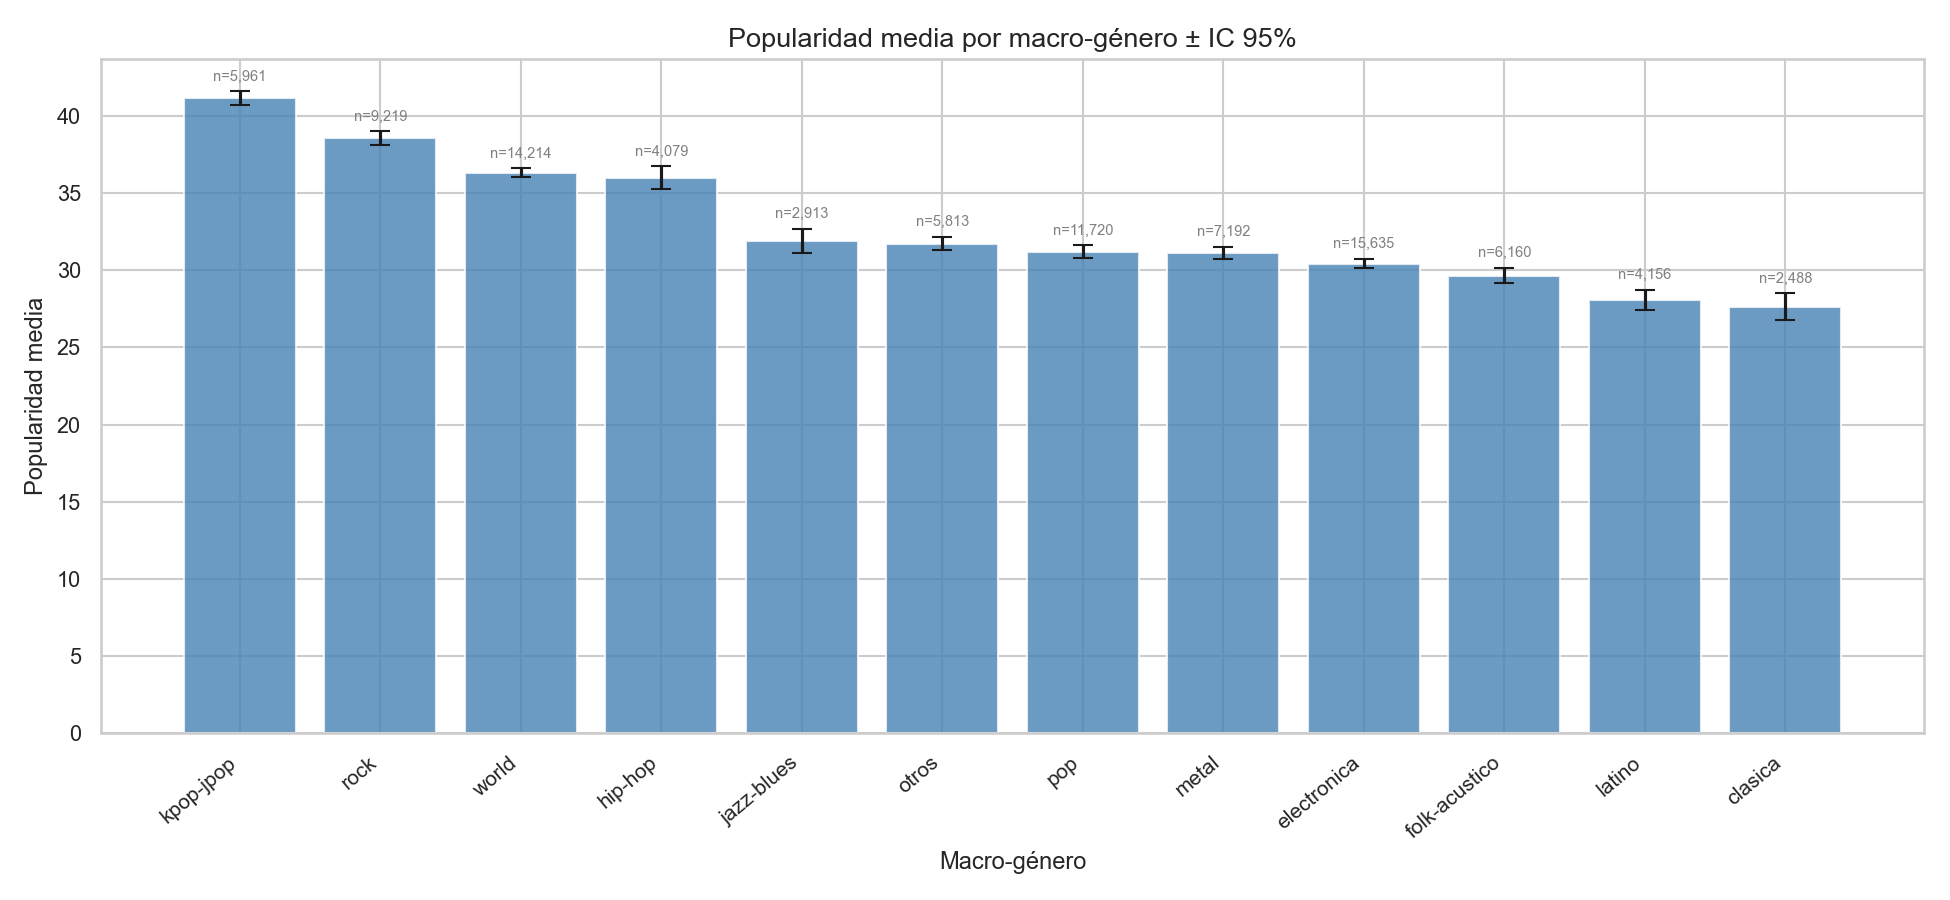
\includegraphics[width=\textwidth]{B7_popularity_by_genre_ci}
  \caption{Popularidad media por macro-género con intervalo de confianza al 95\%.
           El número de canciones por grupo se indica encima de cada barra.}
  \label{fig:B7}
\end{figure}

Dado que los grupos tienen entre 2.488 y 15.635 observaciones, los intervalos de
confianza son muy estrechos y las diferencias entre macro-géneros son
estadísticamente significativas. El K-pop/J-pop encabeza el ranking de popularidad
media (41,2), seguido de la electrónica y el hip-hop. La música clásica (27,6) y
el jazz/blues (29,3) presentan los valores más bajos, principalmente debido al
sesgo de recencia del índice: sus obras más representativas son anteriores a 2010.

\begin{observacion}
Las diferencias de popularidad entre géneros no deben interpretarse como
diferencias de calidad artística o de éxito comercial histórico. Reflejan
principalmente cuándo se produjeron las canciones más escuchadas de cada género
en relación al momento de extracción del dataset (2022).
\end{observacion}

\section{Variables categóricas vs. Popularidad (B.8)}

La Figura~\ref{fig:B8} analiza el efecto de las variables categóricas
\texttt{explicit}, \texttt{mode} y \texttt{key} sobre la popularidad.

\begin{figure}[H]
  \centering
  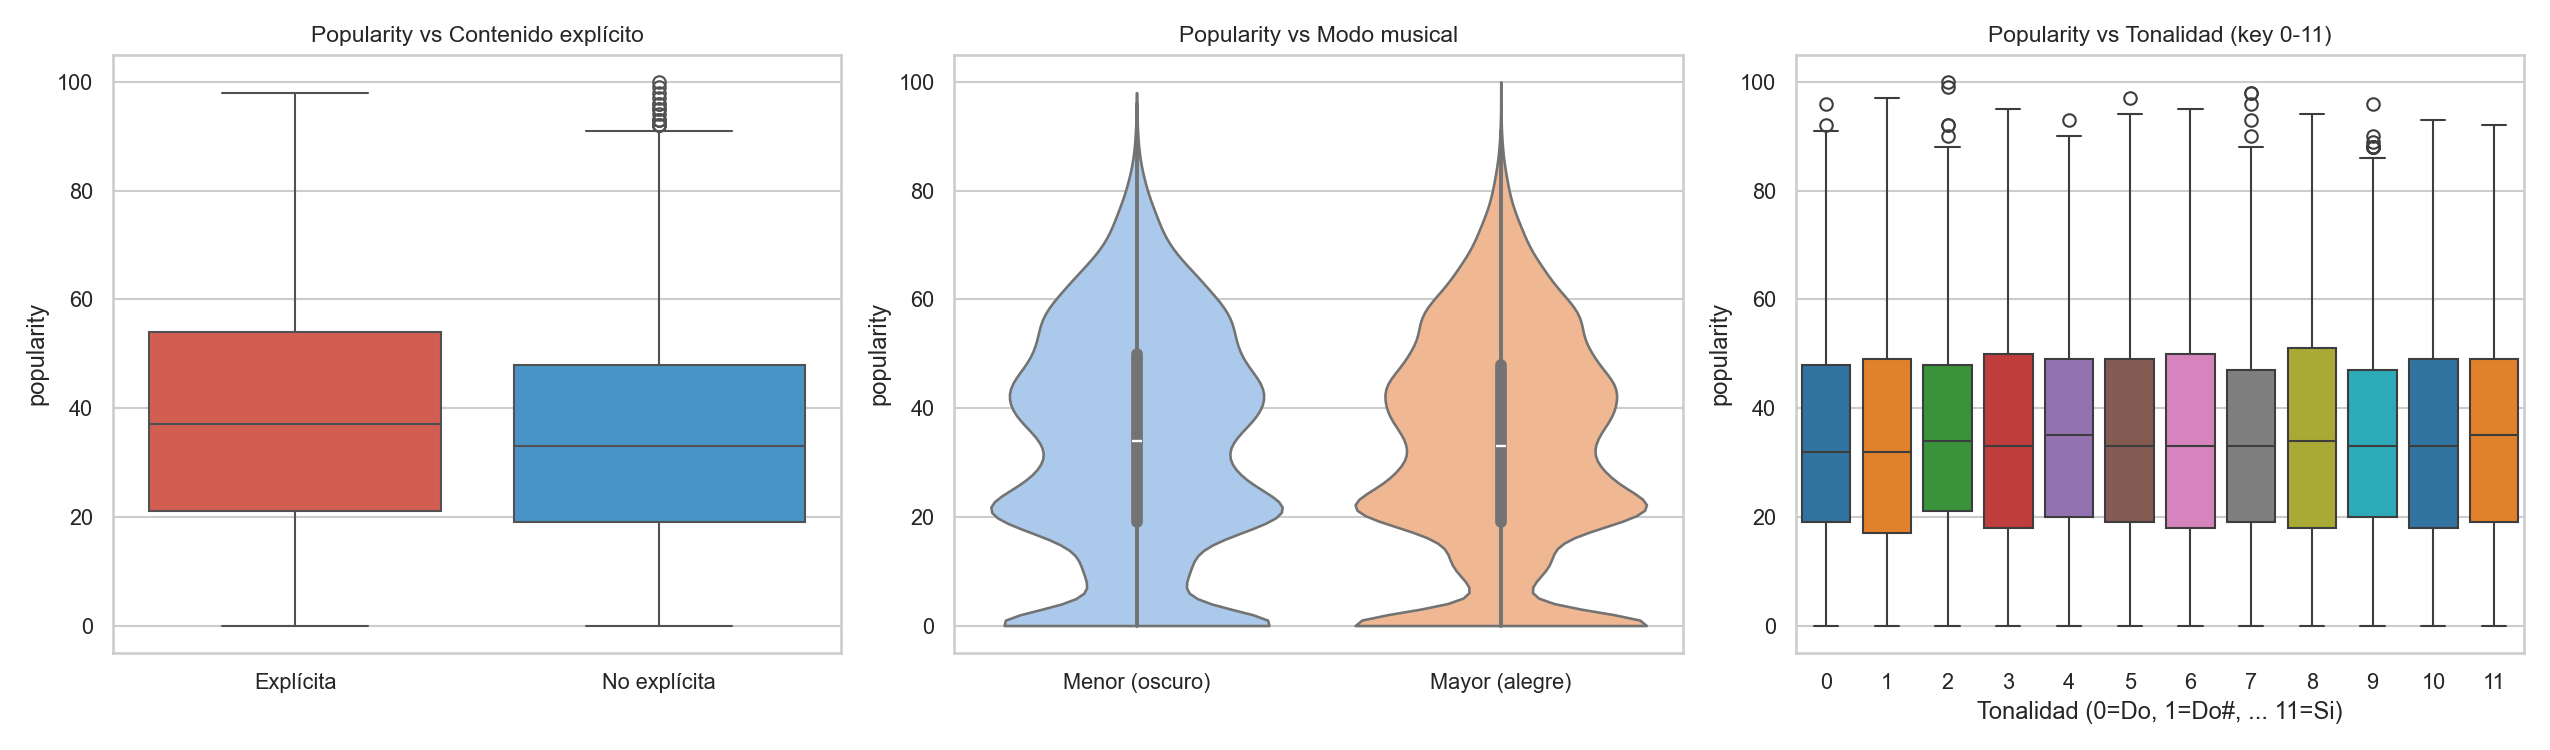
\includegraphics[width=\textwidth]{B8_categorical_vs_popularity}
  \caption{Popularidad según contenido explícito (boxplot), modo musical
           (violin plot) y tonalidad (boxplot por key 0--11).}
  \label{fig:B8}
\end{figure}

Se aplicaron tests estadísticos para cuantificar la significación de las diferencias:

\begin{itemize}
  \item \textbf{Contenido explícito}: test de Mann-Whitney ($p < 0{,}001$).
        Las canciones explícitas tienen una popularidad media significativamente
        mayor. Esto se debe a su asociación con géneros urbanos (hip-hop, trap,
        reggaeton) que dominan los charts del período analizado, no a que el
        contenido explícito per se aumente la popularidad.
  \item \textbf{Modo musical}: test de Mann-Whitney entre Mayor y Menor
        ($p < 0{,}001$, diferencia muy pequeña). Las canciones en modo Mayor
        tienen una mediana de popularidad ligeramente superior.
  \item \textbf{Tonalidad}: ANOVA de un factor ($F = 4{,}74$, $p < 0{,}001$).
        Aunque estadísticamente significativo, el tamaño del efecto es mínimo:
        la variación entre tonalidades explica menos del $0{,}01\%$ de la
        varianza total de popularity. El resultado se debe al elevado tamaño
        muestral, que da potencia estadística incluso a diferencias
        prácticamente irrelevantes.
\end{itemize}

\section{Análisis de los artistas más representados (B.9)}

La Figura~\ref{fig:B9} compara el número de canciones en el dataset y la
popularidad media de los 20 artistas más presentes.

\begin{figure}[H]
  \centering
  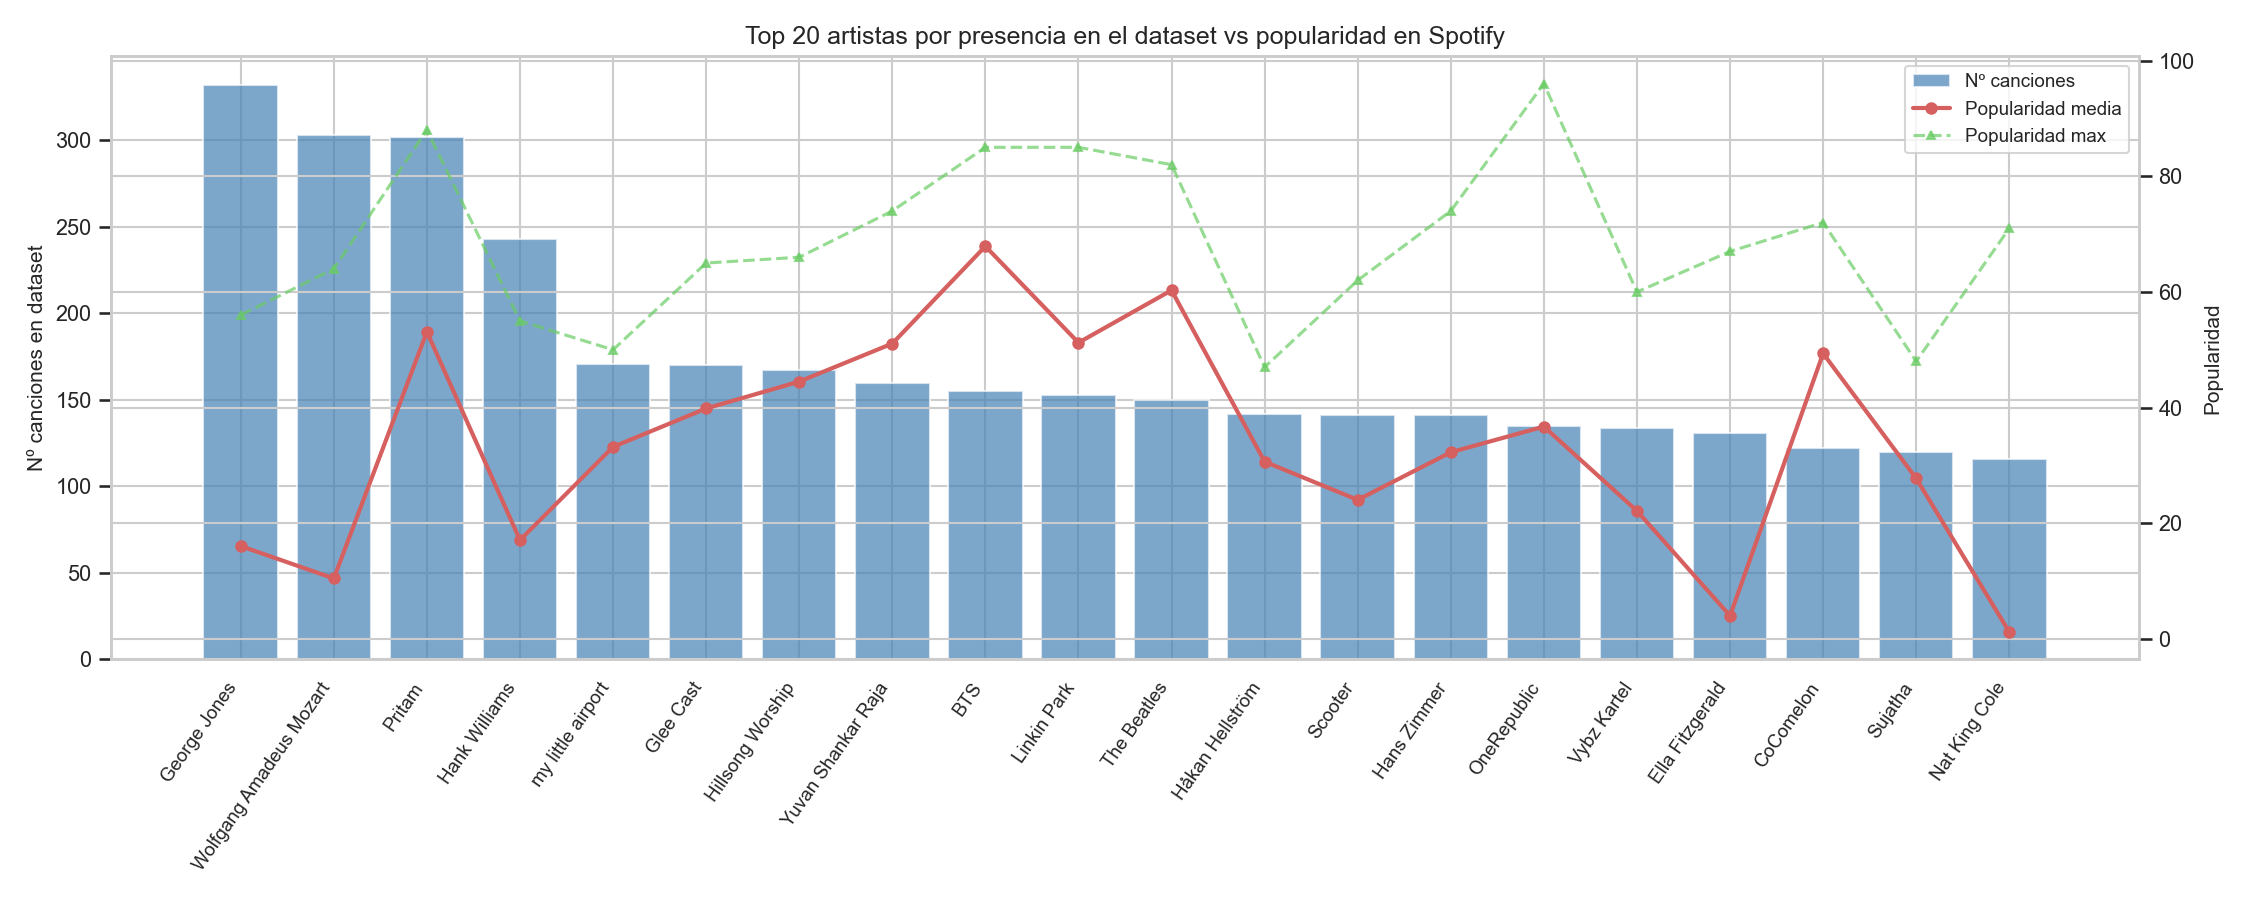
\includegraphics[width=\textwidth]{B9_top_artists}
  \caption{Top 20 artistas por número de canciones en el dataset y su
           popularidad media y máxima en el snapshot de Spotify.}
  \label{fig:B9}
\end{figure}

El gráfico revela una \textbf{paradoja estadística}: los artistas con mayor
presencia en el dataset (The Beatles, George Jones, Stevie Wonder, Linkin Park,
Ella Fitzgerald) no son los más populares en el snapshot. Artistas con catálogos
masivos pero publicados décadas antes de 2022 aparecen con popularidades bajas
porque su actividad de escucha reciente es menor que la de artistas contemporáneos.

Este hallazgo tiene implicaciones directas para cualquier análisis de popularidad
por artista: se está midiendo el \textbf{éxito presente}, no el histórico.

\section{Canciones con popularidad cero (B.10)}

La Figura~\ref{fig:B10} estudia específicamente las 9.410 canciones con
\texttt{popularity}$= 0$.

\begin{figure}[H]
  \centering
  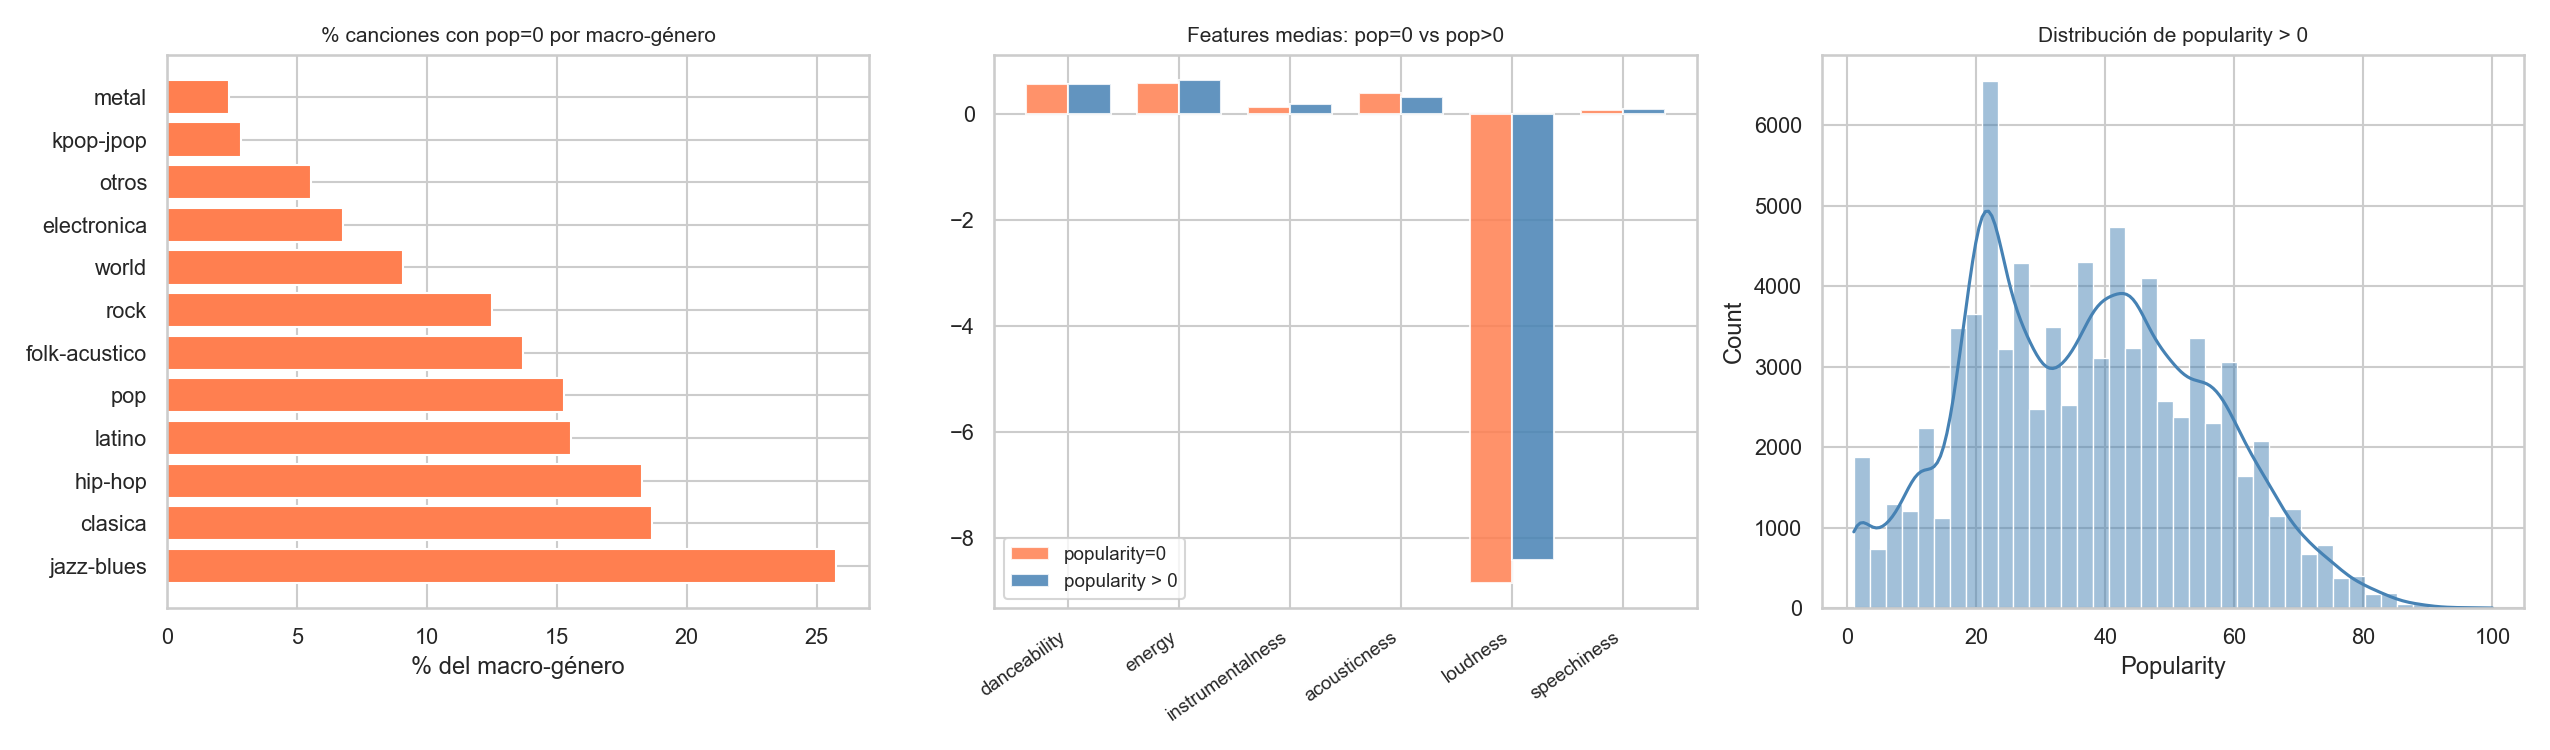
\includegraphics[width=\textwidth]{B10_popularity_zero_analysis}
  \caption{Izquierda: porcentaje de canciones con \texttt{popularity}=0 por
           macro-género. Centro: comparación de features medias entre canciones
           con \texttt{popularity}=0 y \texttt{popularity}>0.
           Derecha: distribución de \texttt{popularity} para canciones con
           \texttt{popularity}>0.}
  \label{fig:B10}
\end{figure}

El jazz/blues tiene la mayor tasa de canciones con popularidad cero (25,7\%),
seguido de la música clásica. Las canciones con \texttt{popularity}$=0$ presentan,
de media:

\begin{itemize}
  \item Mayor \texttt{instrumentalness} ($0{,}124$ vs. $0{,}179$)
  \item Mayor \texttt{acousticness} ($0{,}386$ vs. $0{,}321$)
  \item Menor \texttt{energy} ($0{,}581$ vs. $0{,}641$)
\end{itemize}

Esto confirma que las canciones instrumentales y acústicas de géneros históricos
son las más afectadas por el sesgo de recencia del índice de Spotify.

\section{Resumen de los hallazgos del EDA}

\begin{table}[H]
\centering
\caption{Resumen ejecutivo del Análisis Exploratorio de Datos}
\label{tab:eda_resumen}
\small
\rowcolors{2}{gristabla}{white}
\begin{tabular}{p{3.5cm}p{9.5cm}}
\toprule
\textbf{Variable / análisis} & \textbf{Hallazgo clave} \\
\midrule
\texttt{popularity} &
  Distribución no normal, bimodal. Pico en 0 (10,5\% de canciones).
  Mediana = 33, media = 33,2. \\
\texttt{instrumentalness} &
  Mayor correlación negativa con popularity ($r_S = -0{,}124$).
  Las canciones sin voz son menos populares en el snapshot. \\
\texttt{energy}--\texttt{loudness} &
  Correlación alta ($r_S = +0{,}75$): posible redundancia en modelos lineales,
  irrelevante para \textit{ensemble methods}. \\
\texttt{explicit} &
  Canciones explícitas significativamente más populares (Mann-Whitney $p < 0{,}001$).
  Efecto mediado por el género, no por el contenido per se. \\
\texttt{key} (tonalidad) &
  Sin efecto práctico sobre popularity a pesar de ANOVA $p < 0{,}001$
  (artefacto del tamaño muestral). \\
Macro-género &
  Hip-hop, kpop-jpop y pop $>$ clásica y jazz en popularidad media.
  Efecto principalmente de recencia. \\
Canciones con pop $= 0$ &
  9.410 canciones (10,5\%). Más instrumentales y acústicas. Concentradas
  en jazz-blues y clásica. \\
\bottomrule
\end{tabular}
\end{table}

%% ── CAPÍTULO 4: MODELOS PREDICTIVOS (FASE C) ───────────────
\chapter{Modelos Predictivos: Random Forest y XGBoost}
\label{ch:modelos}

\section{Introducción y enfoque metodológico}

La Fase C aborda dos problemas supervisados sobre el dataset de Spotify:

\begin{enumerate}
  \item \textbf{Regresión de popularidad}: predecir la variable continua
        \texttt{popularity} $\in [0, 100]$ a partir de las features de audio.
  \item \textbf{Clasificación de macro-género}: asignar una canción a uno de los
        12 macro-géneros definidos en la Fase A.
\end{enumerate}

Ambas tareas se abordan con dos familias de modelos de \textit{ensemble} basados
en árboles de decisión: \textbf{Random Forest} y \textbf{XGBoost}. Estos modelos
se eligieron por cuatro razones:

\begin{itemize}
  \item Robustez frente a la multicolinealidad entre features (detectada en la Fase B).
  \item Capacidad de capturar interacciones no lineales sin especificación manual.
  \item Escalabilidad a los 89.550 registros del dataset.
  \item Compatibilidad con el método de explicabilidad SHAP (\textit{TreeExplainer}),
        que asigna contribuciones individuales a cada feature para cada predicción.
\end{itemize}

\section{Preprocesado específico para modelado}

\subsection{Partición estratificada train/test}

Se realizó una partición 80\%/20\% estratificada por macro-género:

$$n_{\text{train}} = 71.640, \quad n_{\text{test}} = 17.910$$

La Figura~\ref{fig:C_split} confirma que las distribuciones de \texttt{popularity}
y la proporción de macro-géneros son equivalentes entre los conjuntos de
entrenamiento y test.

\begin{figure}[H]
  \centering
  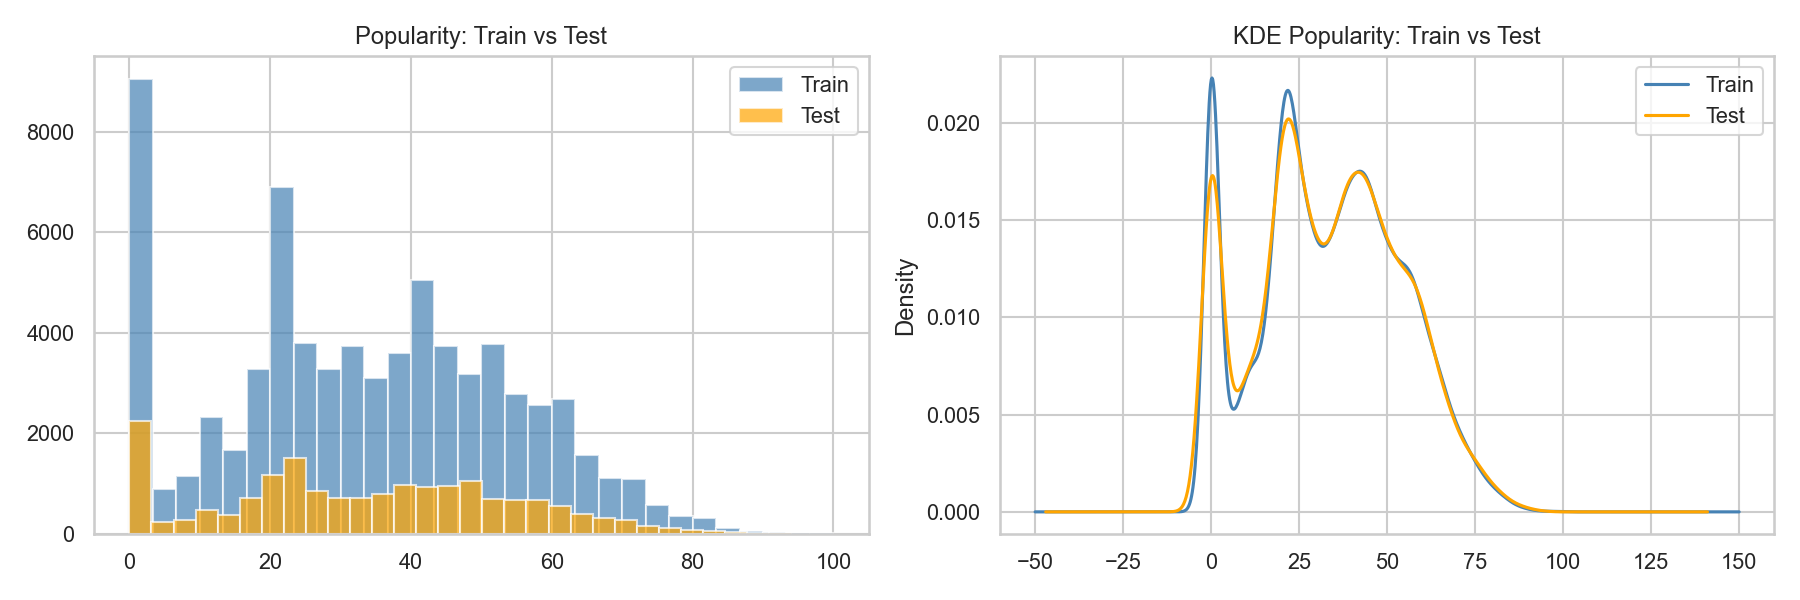
\includegraphics[width=\textwidth]{C_train_test_distribution}
  \caption{Distribución de \texttt{popularity} en train y test
           (histograma superpuesto) y proporciones de macro-género en ambos
           conjuntos. La estratificación garantiza representatividad.}
  \label{fig:C_split}
\end{figure}

\subsection{Codificación de la variable de género con Target Encoding}

Con 114 géneros en \texttt{track\_genre}, la codificación \textit{one-hot}
generaría 114 columnas adicionales y dispersión extrema. Se optó por
\textbf{Target Encoding} (\texttt{TargetEncoder}, biblioteca
\texttt{category\_encoders}): cada categoría se reemplaza por la media de la
variable objetivo calculada \textit{exclusivamente sobre el conjunto de
entrenamiento}, con suavizado de Bayes para categorías con pocas observaciones:

$$\hat{\mu}_c = \frac{n_c \cdot \bar{y}_c + \lambda \cdot \bar{y}}{n_c + \lambda}$$

donde $n_c$ es el número de observaciones de la categoría $c$, $\bar{y}_c$ su
media de \texttt{popularity}, $\bar{y}$ la media global y $\lambda$ el parámetro
de suavizado. El encoder se ajusta únicamente sobre el train para evitar
\textit{data leakage}.

\subsection{Conjunto de features de modelado}

\begin{table}[H]
\centering
\caption{Features utilizadas para la regresión de popularidad}
\label{tab:features_reg}
\small
\rowcolors{2}{gristabla}{white}
\begin{tabular}{ll}
\toprule
\textbf{Feature} & \textbf{Tipo / Origen} \\
\midrule
\texttt{danceability}, \texttt{energy}, \texttt{loudness} & Audio feature original \\
\texttt{speechiness}, \texttt{liveness}, \texttt{valence}, \texttt{tempo} & Audio feature original \\
\texttt{duration\_ms}, \texttt{explicit}, \texttt{key}, \texttt{mode}, \texttt{time\_signature} & Metadata original \\
\texttt{log\_instrumentalness} & Transformación logarítmica (Fase A) \\
\texttt{log\_acousticness} & Transformación logarítmica (Fase A) \\
\texttt{log\_speechiness} & Transformación logarítmica (Fase A) \\
\texttt{electronic\_ratio} & Feature engineered: $\texttt{energy} / (\texttt{acousticness}+0{,}01)$ \\
\texttt{track\_genre} (encoded) & Target encoding sobre train \\
\bottomrule
\end{tabular}
\end{table}

\section{Búsqueda de hiperparámetros}

Dado el tamaño del dataset ($n \approx 90.000$), se empleó
\texttt{RandomizedSearchCV} con 3-fold cross-validation, evaluando 20
combinaciones aleatorias para la regresión y 15 para la clasificación. La
métrica de optimización fue el RMSE negativo (regresión) y el F1-macro
(clasificación).

\begin{table}[H]
\centering
\caption{Espacio de búsqueda de hiperparámetros para Random Forest y XGBoost}
\label{tab:hyperparam}
\small
\begin{tabular}{lll}
\toprule
\textbf{Modelo} & \textbf{Hiperparámetro} & \textbf{Rango / Valores} \\
\midrule
\multirow{4}{*}{Random Forest}
  & \texttt{n\_estimators}      & $\{100, 200, 300\}$ \\
  & \texttt{max\_depth}         & $\{10, 20, 30, \text{None}\}$ \\
  & \texttt{min\_samples\_leaf} & $\{1, 2, 4\}$ \\
  & \texttt{max\_features}      & $\{0{,}3, 0{,}5, 0{,}7, \sqrt{p}\}$ \\
\midrule
\multirow{6}{*}{XGBoost}
  & \texttt{n\_estimators}     & $\{200, 300, 500\}$ \\
  & \texttt{max\_depth}        & $\{4, 6, 8, 10\}$ \\
  & \texttt{learning\_rate}    & $\{0{,}01, 0{,}05, 0{,}1, 0{,}2\}$ \\
  & \texttt{subsample}         & $\{0{,}7, 0{,}8, 1{,}0\}$ \\
  & \texttt{colsample\_bytree} & $\{0{,}7, 0{,}8, 1{,}0\}$ \\
  & \texttt{gamma}             & $\{0, 0{,}1, 0{,}3\}$ \\
\bottomrule
\end{tabular}
\end{table}

Los mejores hiperparámetros encontrados para regresión son:
\begin{itemize}
  \item \textbf{RF}: \texttt{n\_estimators=300}, \texttt{max\_depth=30},
        \texttt{min\_samples\_leaf=2}, \texttt{max\_features=0.5}.
  \item \textbf{XGB}: \texttt{n\_estimators=300}, \texttt{max\_depth=8},
        \texttt{learning\_rate=0.05}, \texttt{subsample=1.0},
        \texttt{colsample\_bytree=0.8}.
\end{itemize}

\section{Resultados de regresión de popularidad}

\subsection{Métricas comparativas}

\begin{table}[H]
\centering
\caption{Métricas de regresión de \texttt{popularity} en el conjunto test ($n = 17.910$)}
\label{tab:reg_metrics}
\rowcolors{2}{gristabla}{white}
\begin{tabular}{lccc}
\toprule
\textbf{Modelo} & \textbf{RMSE} & \textbf{MAE} & \textbf{R\textsuperscript{2}} \\
\midrule
Random Forest    & 14{,}864 & 10{,}160 & 0{,}472 \\
XGBoost          & 15{,}444 & 10{,}841 & 0{,}430 \\
\midrule
\textit{Baseline} (predice siempre la media) & 22{,}3 & 17{,}8 & 0{,}000 \\
\bottomrule
\end{tabular}
\end{table}

El \textbf{Random Forest} supera a XGBoost en todas las métricas. Un
$R^2 = 0{,}472$ significa que el modelo explica el $47{,}2\%$ de la varianza
de \texttt{popularity}; el $52{,}8\%$ restante corresponde a factores externos
al audio no capturados en el dataset: playlists editoriales, campañas de
marketing, viralidad en redes sociales y comportamiento colectivo de los usuarios.

El RMSE de 14{,}864 implica que, de media, la predicción de popularidad difiere
en $\pm 15$ puntos respecto al valor real. En una escala de 0 a 100 esto
representa un error relativo del $\pm 15\%$, aceptable dado que la popularidad
depende en gran medida de factores no observables con los datos disponibles.

\subsection{Curvas de aprendizaje}

La Figura~\ref{fig:C_learning} muestra la evolución del error de entrenamiento y
de validación del Random Forest en función del tamaño del conjunto de entrenamiento.

\begin{figure}[H]
  \centering
  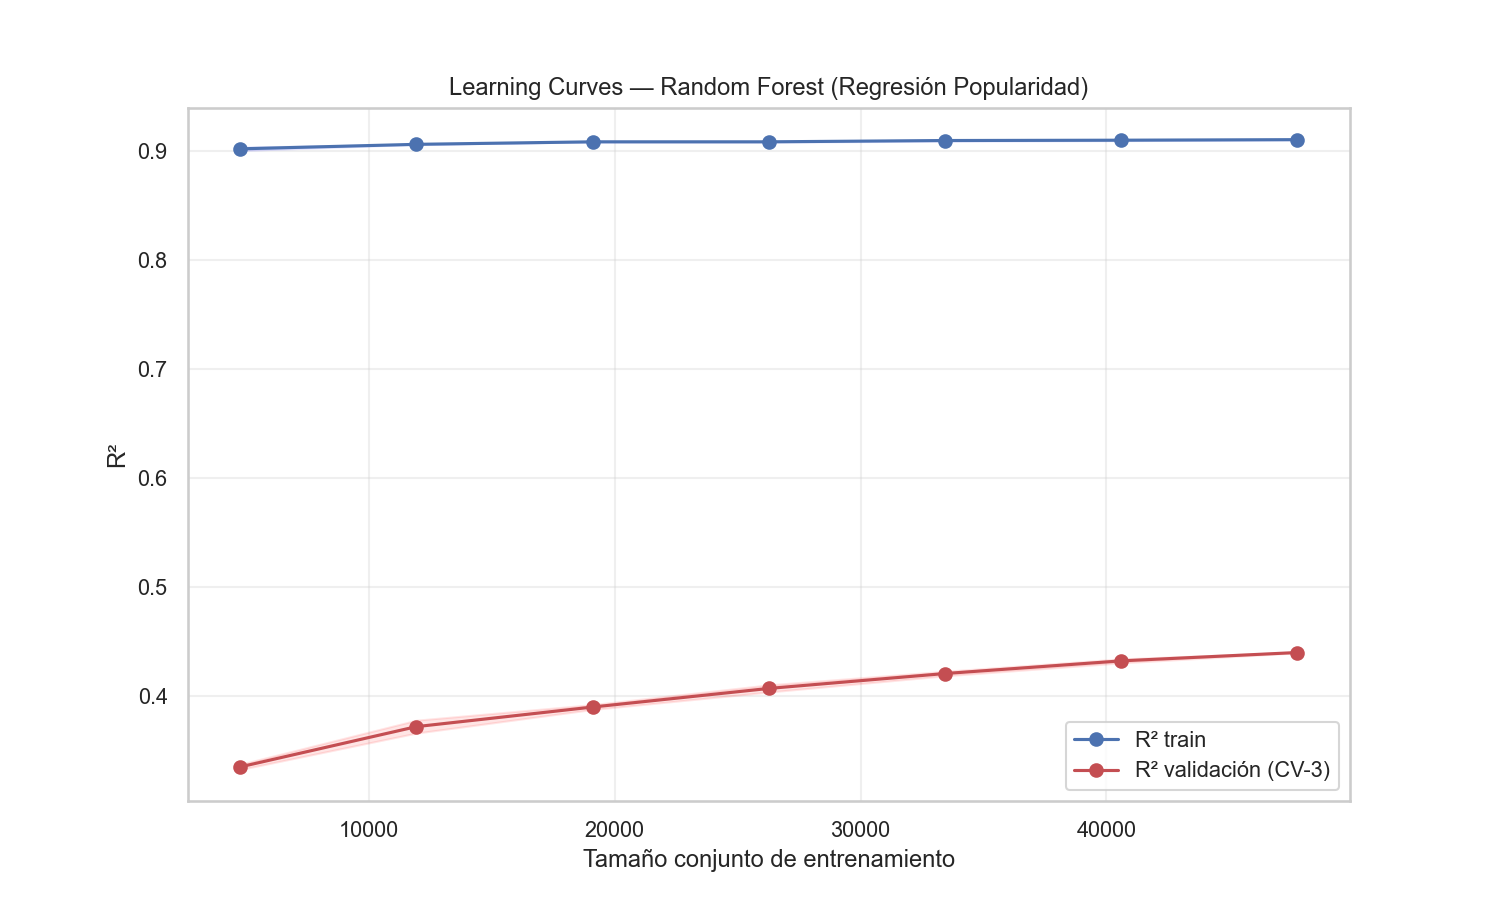
\includegraphics[width=\textwidth]{C_learning_curves_rf}
  \caption{Curvas de aprendizaje del Random Forest para regresión de popularidad.
           Izquierda: RMSE en train (azul) y validación cruzada (naranja) en
           función del número de muestras. Derecha: impacto del porcentaje de
           datos de entrenamiento en el RMSE final de test.}
  \label{fig:C_learning}
\end{figure}

\begin{figure}[H]
  \centering
  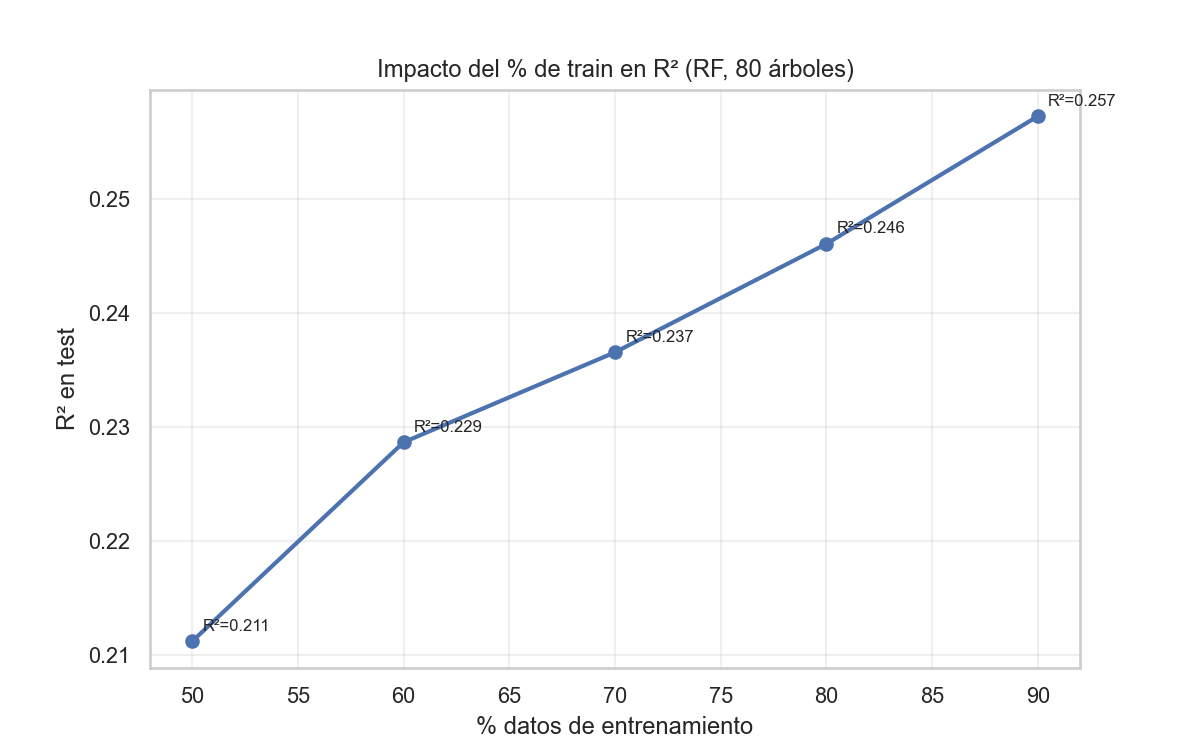
\includegraphics[width=0.85\textwidth]{C_train_size_impact}
  \caption{RMSE en train y test en función del porcentaje del conjunto de
           entrenamiento utilizado. El modelo se estabiliza a partir de
           $\approx 55\%$ de los datos, indicando que el cuello de botella no
           es la cantidad de datos sino la información contenida en las features.}
  \label{fig:C_trainsize}
\end{figure}

Las curvas muestran que el modelo se beneficia de datos adicionales hasta
aproximadamente $n = 50.000$ observaciones; a partir de ahí la mejora
marginal es mínima. El gap moderado entre train y validación indica
overfitting controlado, consistente con los hiperparámetros de regularización
encontrados (\texttt{min\_samples\_leaf=2}, \texttt{max\_features=0.5}).

\subsection{Análisis de residuos}

\begin{figure}[H]
  \centering
  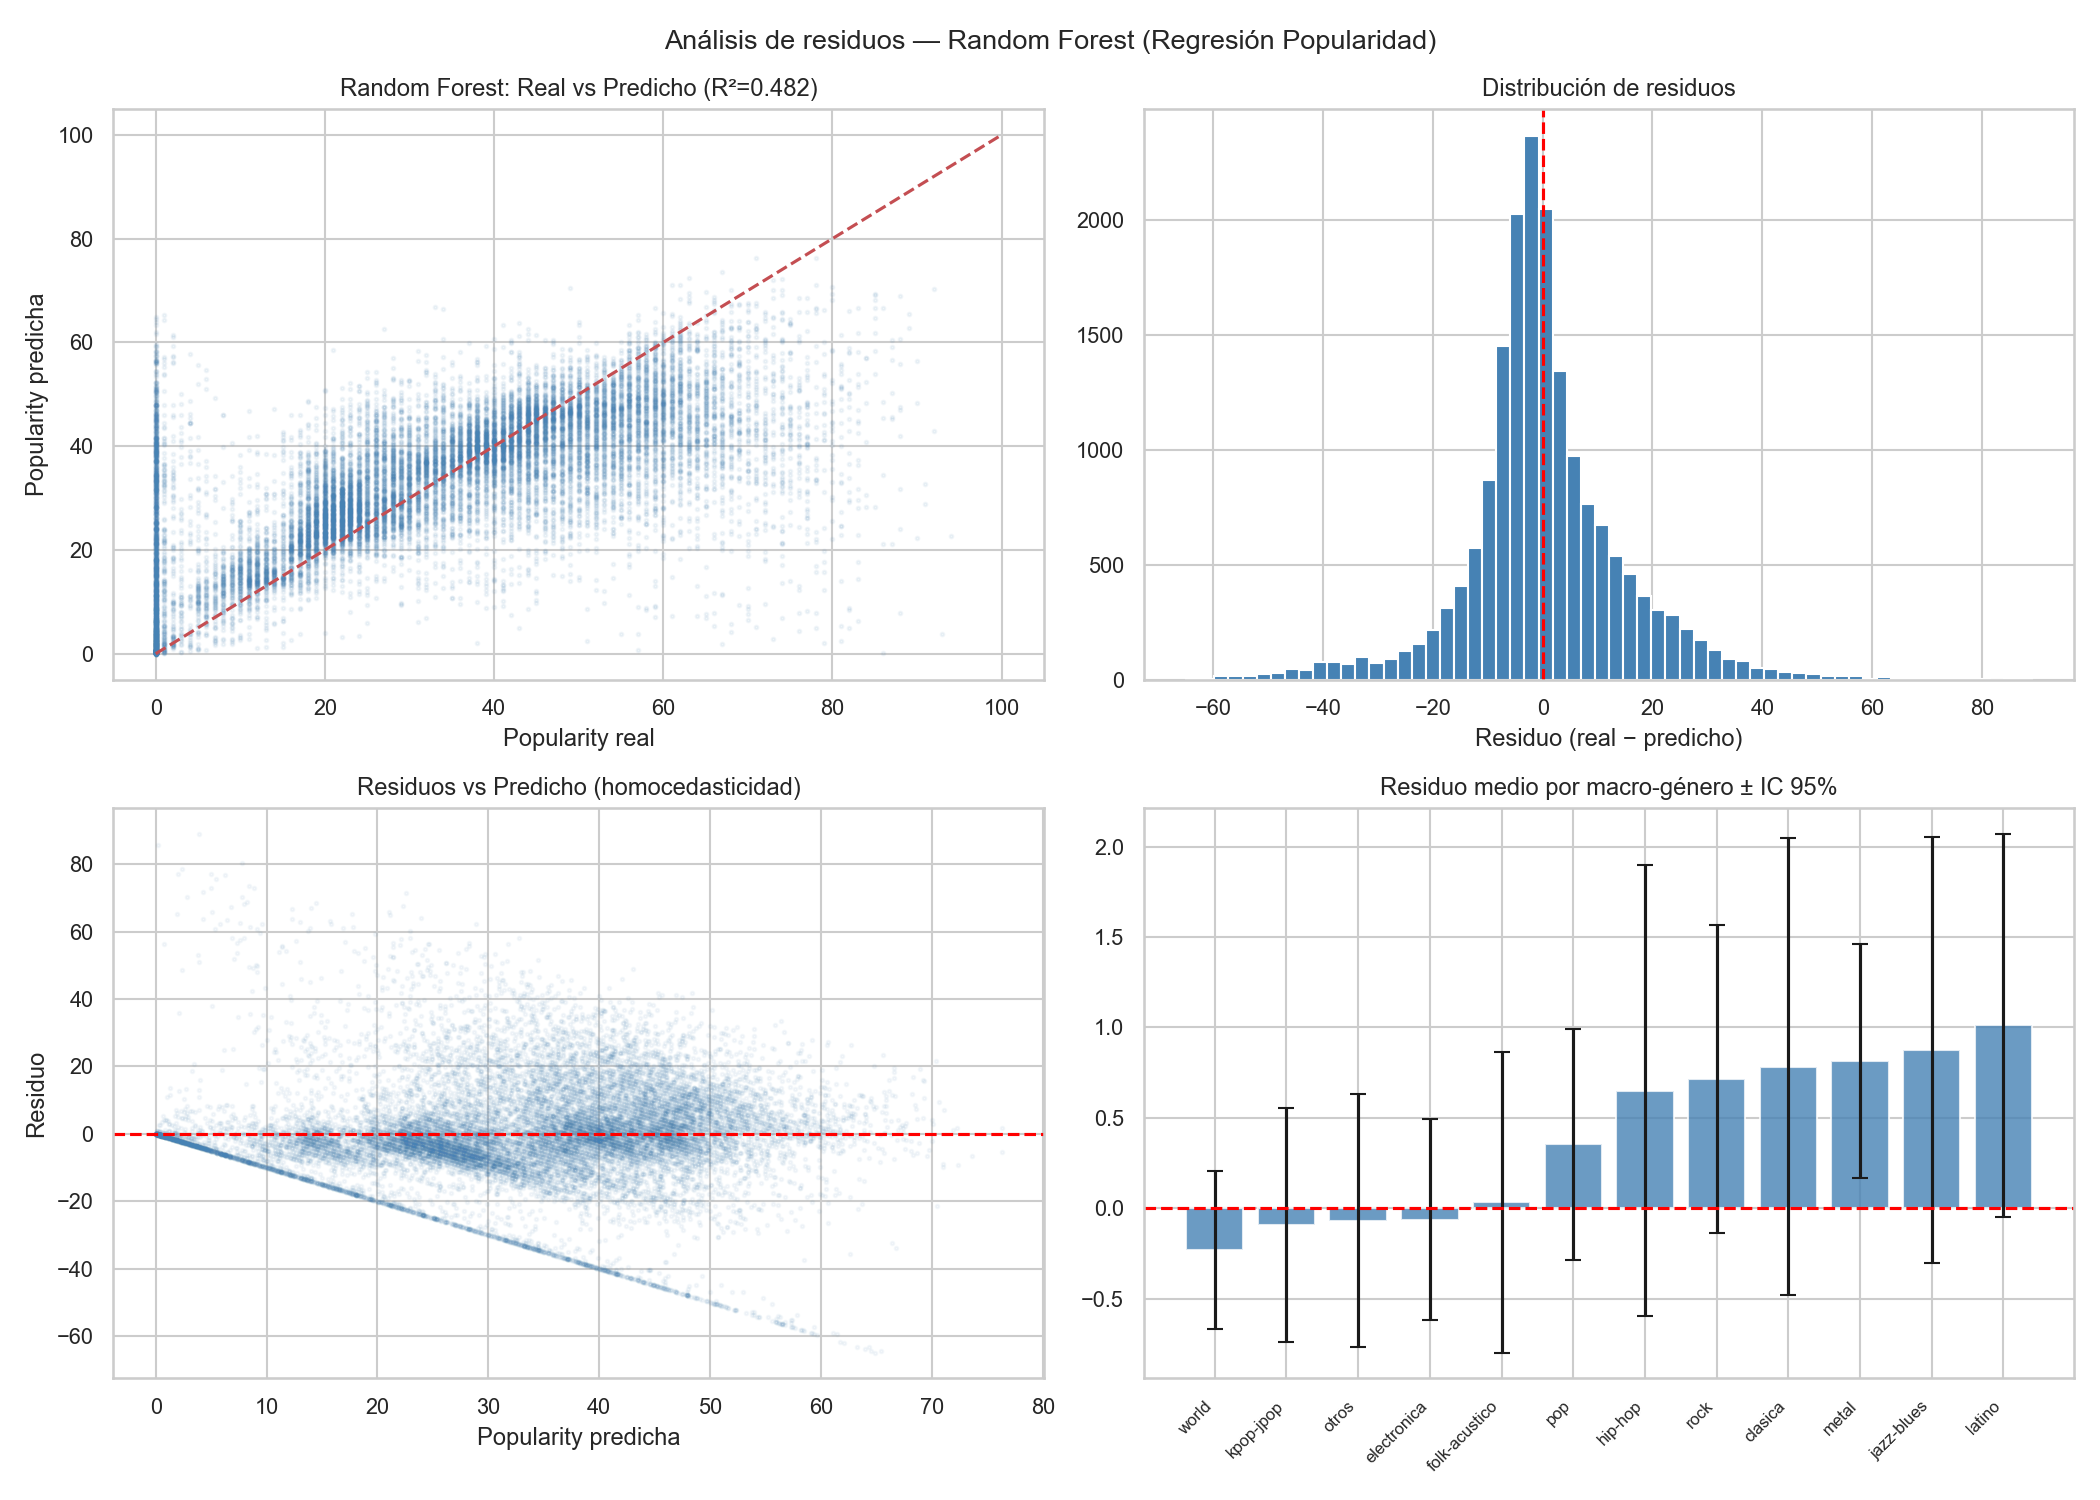
\includegraphics[width=\textwidth]{C_residual_analysis}
  \caption{Análisis de residuos del Random Forest (regresión de popularidad).
           Paneles: distribución de residuos, residuos vs.\ predicción,
           residuos vs.\ valor real y Q-Q plot de residuos.}
  \label{fig:C_residuals}
\end{figure}

El análisis de residuos revela dos sesgos sistemáticos:

\begin{enumerate}
  \item \textbf{Sobreestimación de canciones con \texttt{popularity}~$= 0$}:
        el modelo predice valores positivos para muchas canciones con popularidad
        real cero, porque aprende la media condicionada a las features.
  \item \textbf{Subestimación en popularidades muy altas} ($>$ 80): los valores
        extremos de popularidad están impulsados por factores externos al audio
        que el modelo no puede capturar; tiende a predecir valores de
        popularidad media-alta para estas canciones.
\end{enumerate}

\section{Explicabilidad con valores SHAP}

Los valores SHAP (\textit{SHapley Additive exPlanations}, Lundberg \& Lee, 2017)
permiten descomponer cualquier predicción individual del modelo como suma de
contribuciones aditivas de cada feature:

$$\hat{f}(x) = \phi_0 + \sum_{j=1}^{p} \phi_j(x)$$

donde $\phi_0$ es el valor base (media de todas las predicciones sobre el train)
y $\phi_j(x)$ es la contribución de la feature $j$ a la predicción para el
ejemplo $x$. Los valores SHAP se calcularon con \texttt{TreeExplainer} sobre una
muestra aleatoria de 1.000 observaciones del test.

\begin{figure}[H]
  \centering
  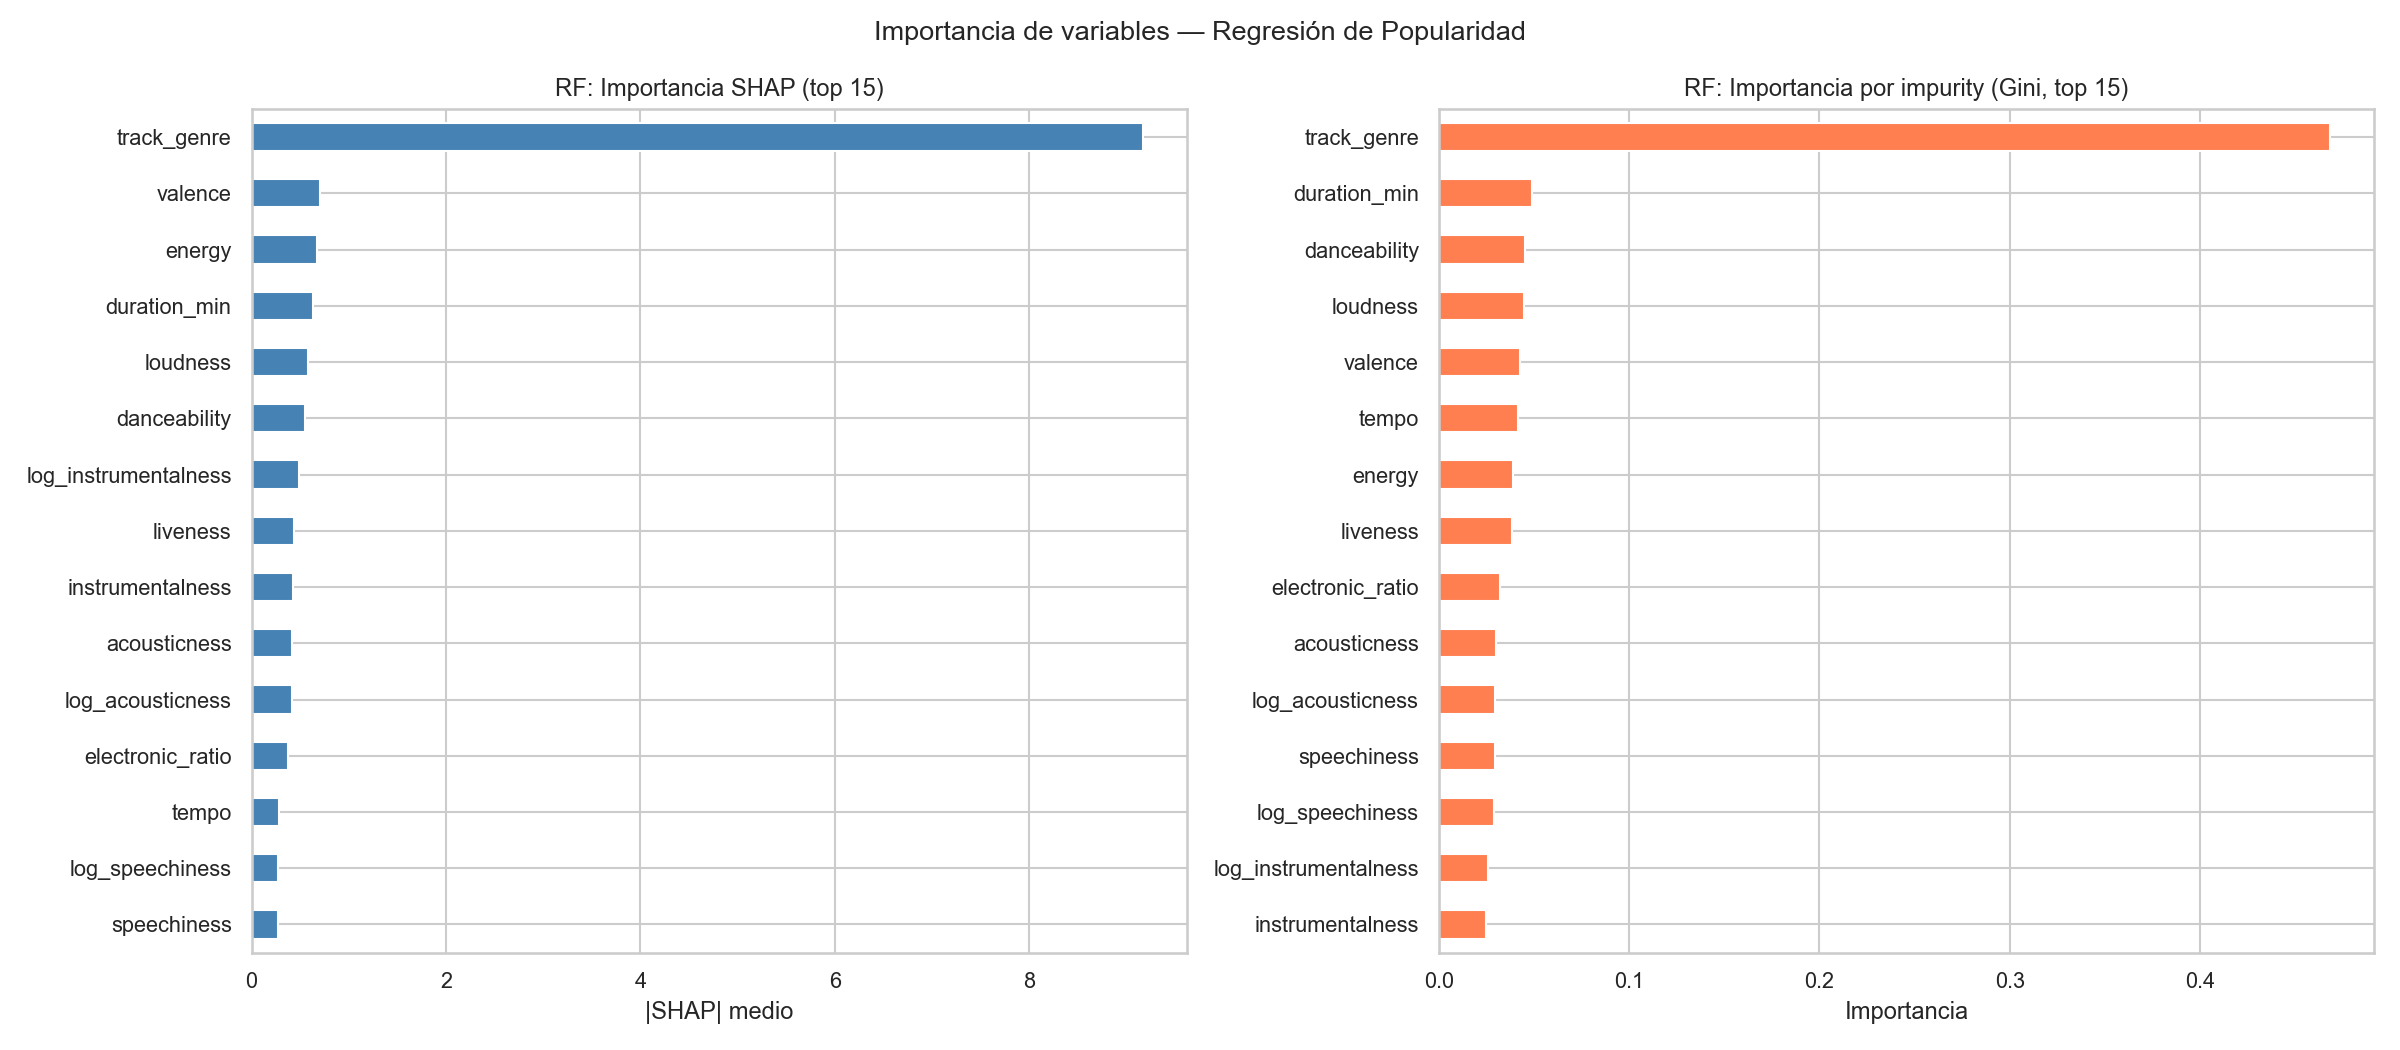
\includegraphics[width=\textwidth]{C_shap_importance_reg}
  \caption{Importancia de features según valores SHAP para la regresión de
           popularidad (Random Forest). Barra: media del valor absoluto SHAP.
           Se compara con la importancia por impureza (Gini) para mostrar las
           diferencias entre ambos métodos de explicabilidad.}
  \label{fig:C_shap_imp}
\end{figure}

\begin{figure}[H]
  \centering
  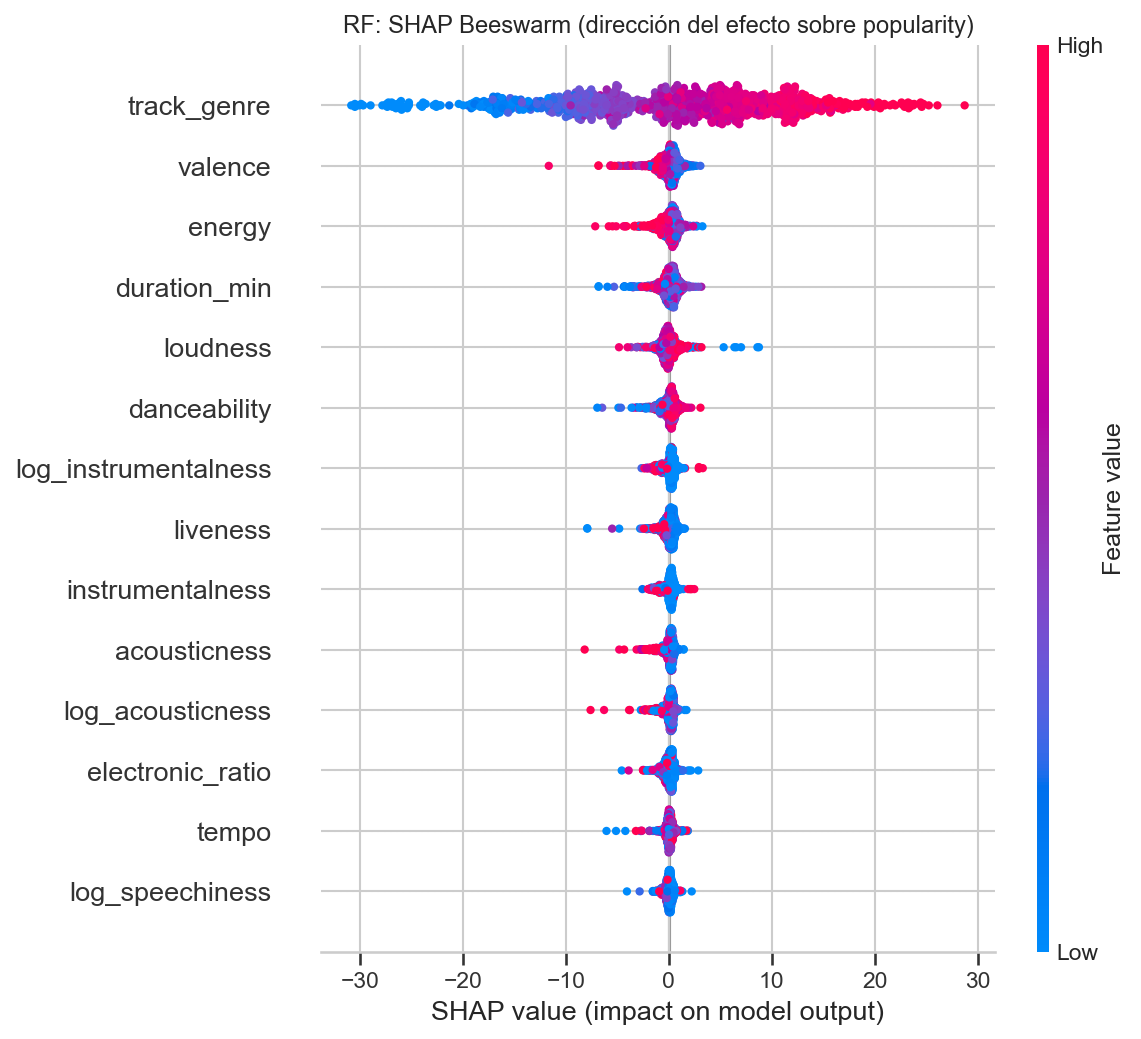
\includegraphics[width=\textwidth]{C_shap_beeswarm_reg}
  \caption{Beeswarm plot de valores SHAP para la regresión de popularidad.
           Cada punto es una observación del test. El eje X indica la
           contribución a la predicción: valores positivos aumentan
           \texttt{popularity} predicha, negativos la reducen. El color
           codifica el valor de la feature (rojo = alto, azul = bajo).}
  \label{fig:C_shap_bee}
\end{figure}

Los resultados SHAP revelan:

\begin{itemize}
  \item \textbf{\texttt{track\_genre} (codificado)} es la feature más influyente:
        el género de la canción tiene mayor capacidad predictiva de popularidad
        que cualquier feature de audio individual, confirmando que el contexto
        cultural domina sobre las características acústicas.
  \item \textbf{\texttt{acousticness}}: valores altos (música acústica) reducen
        la popularidad predicha; valores bajos (música electrónica/urbana) la
        aumentan. Coherente con la correlación de Spearman detectada en la Fase B.
  \item \textbf{\texttt{instrumentalness}}: actúa en la misma dirección; canciones
        con voz (valores bajos) predicen mayor popularidad.
  \item \textbf{\texttt{explicit}}: contribución positiva sistemática mediada
        por la asociación con géneros urbanos populares (hip-hop, trap, reggaeton).
  \item Las \textbf{transformaciones logarítmicas} aportan información
        complementaria a las variables originales, justificando su inclusión.
\end{itemize}

\begin{observacion}
La diferencia entre importancia SHAP e importancia por impureza (Gini) es
metodológicamente relevante: la impureza tiende a sobreestimar la importancia
de variables continuas con muchos valores posibles (como \texttt{duration\_ms}),
mientras que SHAP mide la contribución real promediada sobre todos los órdenes
de introducción de features (valores de Shapley del juego cooperativo). Para
interpretación causal, SHAP es el método preferido.
\end{observacion}

\section{Resultados de clasificación de macro-género}

\subsection{Baseline con 114 géneros sin agrupar}

Se entrenó un Random Forest sin tuning sobre los 114 géneros originales como
referencia de comparación:

\begin{table}[H]
\centering
\caption{Baseline de clasificación con 114 géneros sin agrupación editorial}
\label{tab:baseline_clf}
\begin{tabular}{lcc}
\toprule
\textbf{Modelo} & \textbf{Accuracy} & \textbf{F1-macro} \\
\midrule
RF sin tuning (114 géneros) & 0{,}257 & 0{,}246 \\
\bottomrule
\end{tabular}
\end{table}

Los valores son bajos pero esperables: con 114 clases solapadas estilísticamente
(las features de audio no distinguen ``indie'' de ``indie-pop'') el problema es
estadísticamente difícil. Este baseline sirve de referencia para cuantificar la
mejora obtenida con la agrupación editorial.

\subsection{Clasificación con 12 macro-géneros}

Tras aplicar el mapa editorial de la Fase A y el ajuste de hiperparámetros
con \texttt{RandomizedSearchCV}:

\begin{table}[H]
\centering
\caption{Métricas de clasificación de macro-género (12 clases) en test}
\label{tab:clf_metrics}
\rowcolors{2}{gristabla}{white}
\begin{tabular}{lccr}
\toprule
\textbf{Modelo} & \textbf{Accuracy} & \textbf{F1-macro} & \textbf{Mejora vs.\ baseline} \\
\midrule
Random Forest & 0{,}465 & 0{,}408 & $+66\%$ en F1 \\
XGBoost       & 0{,}464 & 0{,}409 & $+66\%$ en F1 \\
\midrule
\textit{Azar} (uniforme) & $1/12 \approx 0{,}083$ & $0{,}083$ & --- \\
\bottomrule
\end{tabular}
\end{table}

Ambos modelos obtienen resultados prácticamente idénticos, con un F1-macro
de $\approx 0{,}41$ que supera el azar en un factor $\times 5$ y mejora el
baseline (114 géneros sin agrupar) en un $+66\%$.

Los mejores hiperparámetros para clasificación fueron:
\begin{itemize}
  \item \textbf{RF}: \texttt{n\_estimators=300}, \texttt{max\_depth=30},
        \texttt{min\_samples\_leaf=1}, \texttt{max\_features=log2}.
  \item \textbf{XGB}: \texttt{n\_estimators=500}, \texttt{max\_depth=8},
        \texttt{learning\_rate=0.05}, \texttt{subsample=0.7},
        \texttt{colsample\_bytree=0.7}.
\end{itemize}

\subsection{Features más discriminativas en clasificación}

Las tres features más importantes en la tarea de clasificación son:

\begin{itemize}
  \item \textbf{\texttt{acousticness}} (RF y XGB): discrimina clásica/folk
        (alta) de metal/electrónica (baja) con claridad.
  \item \textbf{\texttt{danceability}} (RF): separa géneros bailables (latino,
        kpop) de los no bailables (clásica, ambient).
  \item \textbf{\texttt{instrumentalness}} (XGB): clave para separar clásica y
        ambient (sin voz) del resto de géneros.
\end{itemize}

Este perfil de importancias es plenamente coherente con el gráfico radar de
la Fase B (Figura~\ref{fig:B6}), lo que valida la consistencia interna entre
el análisis exploratorio y los modelos supervisados: las mismas features que
visualmente separan los géneros en el radar son las que el modelo aprende a
usar como señal discriminativa.

\section{Síntesis y discusión}

\begin{table}[H]
\centering
\caption{Síntesis de resultados de la Fase C}
\label{tab:discusion_C}
\small
\rowcolors{2}{gristabla}{white}
\begin{tabular}{p{3.2cm}p{3.8cm}p{6cm}}
\toprule
\textbf{Aspecto} & \textbf{Resultado} & \textbf{Interpretación} \\
\midrule
$R^2$ regresión & 0{,}47 (RF) & El audio explica la mitad de la popularidad;
  el resto depende de factores externos (marketing, playlists, viralidad). \\
F1-macro clasificación & 0{,}41 (12 clases, RF) & Buena discriminación en macro-géneros
  acústicamente diferenciados (clásica, metal); menor en géneros solapados (pop, rock). \\
Diferencia RF vs.\ XGB & Mínima & Ambos capturan estructuras similares; RF
  ligeramente superior en regresión. \\
Sobreajuste & Controlado & Curvas de aprendizaje muestran gap moderado. \\
Feature más influyente & \texttt{track\_genre} (SHAP) & El género codificado aporta
  más información que las features de audio, reflejando la importancia del contexto
  cultural sobre las características acústicas en el algoritmo de Spotify. \\
\bottomrule
\end{tabular}
\end{table}

%% ── CAPÍTULO 5: CLUSTERING Y RECOMENDACIÓN (FASE D) ────────
\chapter{Clustering y Sistema de Recomendación Musical}
\label{ch:clustering}

\section{Introducción: el problema de recomendación musical}

Los sistemas de recomendación de Spotify combinan tres pilares:
(i) \textbf{filtrado colaborativo} (comportamiento de usuarios similares),
(ii) \textbf{análisis de audio} mediante redes neuronales sobre espectrogramas
y (iii) \textbf{NLP} sobre letras, metadatos y blogs. El dataset disponible
no contiene datos de usuarios ni texto, por lo que el sistema que se construye
en esta fase es un \textbf{recomendador basado en contenido (\textit{content-based})},
usando las audio features como proxy del ``embedding de audio'' de Spotify.

Esta restricción se asume explícitamente como limitación del trabajo y la replica
la pieza del sistema de Spotify que sí es reproducible con datos de audio públicos.

\section{Preprocesado para clustering}

\subsection{Selección de features y escalado}

Se seleccionaron las nueve features de audio con mayor varianza interpretativa:
\texttt{danceability}, \texttt{energy}, \texttt{loudness}, \texttt{speechiness},
\texttt{acousticness}, \texttt{instrumentalness}, \texttt{liveness},
\texttt{valence} y \texttt{tempo}.

Las features se escalaron con \texttt{StandardScaler} (media 0, desviación
típica 1) antes de cualquier algoritmo de clustering, ya que las distancias
euclídeas son sensibles a las unidades de medida (\texttt{loudness} está en
dB, \texttt{tempo} en BPM, mientras que el resto son ratios entre 0 y 1).

\subsection{Reducción de dimensionalidad para visualización}

Se aplicó PCA a 2 componentes para permitir la visualización del espacio de
clustering:

$$\text{PC1 explica el } 32{,}0\%, \quad \text{PC2 explica el } 16{,}0\%, \quad
\text{total } = 48{,}0\%$$

Solo el 48\% de la varianza se captura en 2 dimensiones, lo que indica que
el espacio de audio features no tiene una estructura de baja dimensión
simple. Esto es coherente con la fragmentación de géneros observada en la
Fase B.

\section{Comparativa de algoritmos de clustering}

\begin{table}[H]
\centering
\caption{Comparativa de algoritmos de clustering sobre el dataset de audio}
\label{tab:clustering}
\rowcolors{2}{gristabla}{white}
\begin{tabular}{llcc}
\toprule
\textbf{Algoritmo} & \textbf{Configuración} & \textbf{Silhouette} & \textbf{Davies-Bouldin} \\
\midrule
KMeans            & $k = 2$              & 0{,}258 & 1{,}573 \\
Agglomerativo (Ward) & $k = 2$ (10k muestra) & 0{,}185 & 1{,}865 \\
DBSCAN            & $\varepsilon = 1{,}30$, minPts$=10$ (5k muestra) & $-0{,}037$ & 1{,}044 \\
\bottomrule
\end{tabular}
\end{table}

El \textbf{coeficiente de silhouette} mide la cohesión intra-cluster y la
separación inter-cluster en $[-1, 1]$; valores más altos indican clusters
mejor definidos. El \textbf{índice Davies-Bouldin} mide la razón media entre
dispersión interna y separación externa; valores menores son mejores.

\textbf{KMeans con $k = 2$} obtiene el mayor silhouette y se elige para el
sistema de recomendación por su equilibrio entre rendimiento, interpretabilidad
y la capacidad de asignar nuevas canciones a un cluster (método \texttt{predict}).

El análisis de los géneros más representados en cada cluster revela:
\begin{itemize}
  \item \textbf{Cluster 0} (energético): géneros con alta energy y baja
        acousticness --- happy, forro, breakbeat, chicago-house, heavy-metal.
  \item \textbf{Cluster 1} (tranquilo/acústico): géneros con baja energy y
        alta acousticness/instrumentalness --- sleep, ambient, new-age, classical.
\end{itemize}

La convergencia a solo 2 clústeres óptimos es un hallazgo significativo: refleja
que el espacio de features de Spotify está dominado por el eje
``electronización vs. acústica'', la misma dimensión detectada como la pareja de
mayor correlación en la Fase B (energy--acousticness, $r_S = -0{,}71$).

\begin{figure}[H]
  \centering
  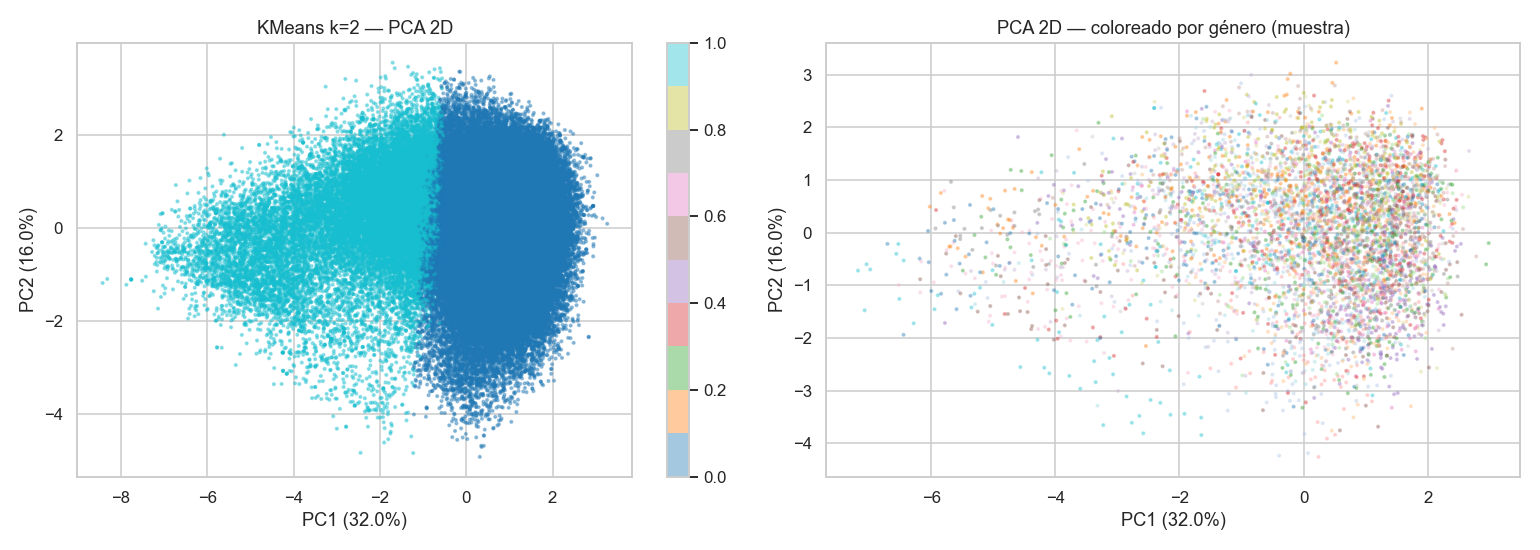
\includegraphics[width=\textwidth]{03b_pca2d_clusters}
  \caption{Visualización PCA 2D del espacio de audio features coloreado por
           cluster KMeans ($k=2$). Las dos nubes corresponden al eje energético
           (PC positivo) vs.\ acústico (PC negativo).}
  \label{fig:D_pca}
\end{figure}

\begin{figure}[H]
  \centering
  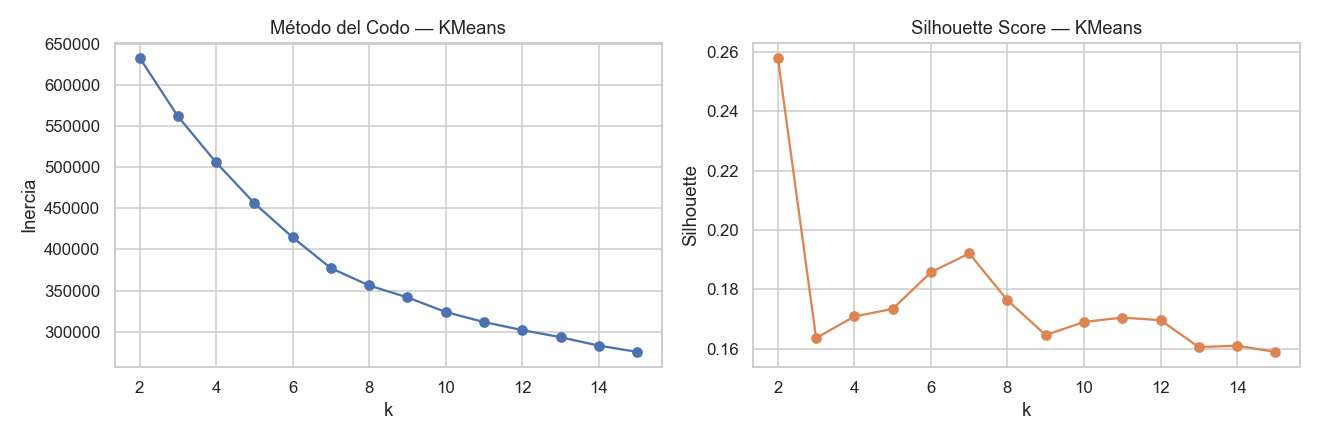
\includegraphics[width=\textwidth]{03a_kmeans_elbow}
  \caption{Método del codo (inercia vs.\ $k$) y silhouette score vs.\ $k$
           para la selección del número óptimo de clusters en KMeans.
           El codo se localiza en $k = 2$.}
  \label{fig:D_elbow}
\end{figure}

\section{Sistema de recomendación musical}

Se implementaron y compararon tres estrategias de recomendación:

\begin{enumerate}
  \item \textbf{KNN global} (vecinos más cercanos en similitud coseno sobre el
        espacio de features escaladas): dada una canción semilla, devuelve las
        $N$ canciones con mayor similitud coseno del dataset.
  \item \textbf{Basado en cluster}: devuelve canciones aleatorias del mismo
        cluster KMeans que la semilla.
  \item \textbf{Híbrido (género + KNN)}: filtra primero por macro-género y luego
        aplica KNN dentro de ese subconjunto, priorizando coherencia estilística
        y similitud sonora.
\end{enumerate}

\subsection{Métricas de evaluación proxy}

La ausencia de \textit{ground truth} real (qué canciones gustan de verdad a cada
usuario) obliga a utilizar métricas proxy calculadas sobre 200 canciones semilla
aleatorias y $N = 10$ recomendaciones por semilla:

\begin{itemize}
  \item \textbf{Coherencia de género}: fracción de recomendaciones que comparten
        el macro-género de la semilla.
  \item \textbf{Diversidad de artistas}: proporción de artistas distintos entre
        las $N$ recomendaciones (1 = todos distintos, 0 = todos iguales).
  \item \textbf{Popularidad media}: media de \texttt{popularity} de las
        recomendaciones.
\end{itemize}

\subsection{Comparativa de los tres recomendadores}

\begin{table}[H]
\centering
\caption{Métricas comparativas de los tres enfoques de recomendación}
\label{tab:recommenders}
\rowcolors{2}{gristabla}{white}
\begin{tabular}{lccc}
\toprule
\textbf{Enfoque} & \textbf{Coherencia género} & \textbf{Diversidad artistas} & \textbf{Pop.\ media} \\
\midrule
KNN global (coseno)  & 0{,}136 & 0{,}871 & 31{,}8 \\
Basado en cluster    & 0{,}125 & 0{,}864 & 32{,}2 \\
Híbrido (género+KNN) & \textbf{1{,}000} & 0{,}831 & 33{,}5 \\
\bottomrule
\end{tabular}
\end{table}

\begin{figure}[H]
  \centering
  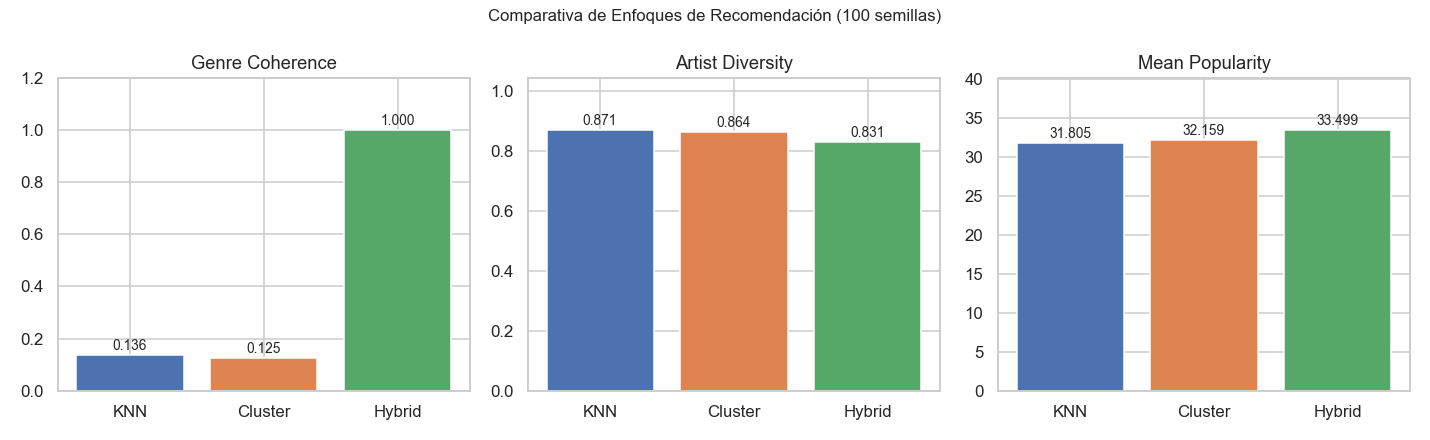
\includegraphics[width=\textwidth]{03d_recommender_comparison}
  \caption{Comparativa visual de las tres métricas de evaluación proxy para los
           tres sistemas de recomendación.}
  \label{fig:D_recommenders}
\end{figure}

Los resultados permiten extraer tres conclusiones:

\begin{enumerate}
  \item El \textbf{recomendador híbrido} alcanza una coherencia de género
        perfecta (1{,}0): todas las canciones recomendadas pertenecen al mismo
        macro-género que la semilla. Esto se debe al filtrado previo por género
        que restringe el espacio de búsqueda KNN. Presenta la menor diversidad
        de artistas (0{,}83), aunque sigue siendo alta.
  \item El \textbf{KNN global} es el más diverso (0{,}87) pero la coherencia de
        género es baja (0{,}14): el espacio de features compartido entre géneros
        hace que los vecinos más cercanos puedan pertenecer a géneros distintos.
        Por ejemplo, una balada rock y una balada pop tienen features similares.
  \item El \textbf{recomendador basado en cluster} tiene el peor rendimiento en
        ambas métricas, ya que con solo 2 clústeres (energético vs.\ acústico)
        la granularidad es insuficiente para recomendaciones específicas de género.
\end{enumerate}

\subsection{Selección para la aplicación final}

Se selecciona el \textbf{enfoque híbrido} como recomendador principal de la
aplicación Streamlit (Fase 4, no desarrollada en este documento) y el KNN global
como alternativa configurable por el usuario cuando se prefiere mayor diversidad
estilística.

\section{Síntesis de la Fase D}

La Fase D muestra que el espacio de audio features de Spotify:

\begin{enumerate}
  \item Tiene una estructura de clustering dominada por el eje
        energético/acústico ($k = 2$ óptimo), no por los géneros musicales
        tal como los entiende la cultura popular.
  \item Permite construir un recomendador basado en contenido con coherencia de
        género perfecta cuando se combina el filtrado por macro-género con KNN,
        replicando la componente de análisis de audio del sistema de Spotify.
  \item Tiene limitaciones inherentes para recomendación cross-genre: la
        similitud coseno en el espacio de audio features mezcla géneros con
        perfiles acústicos parecidos (ballads de distintos géneros, EDM de
        distintos subgéneros).
\end{enumerate}

%% ── CAPÍTULO 6: CONCLUSIONES ────────────────────────────────
\chapter{Conclusiones y Trabajo Futuro}

\section{Conclusiones generales}

Este Trabajo de Fin de Grado ha desarrollado un ciclo completo de \textit{Data
Science} aplicado a la industria musical, desde la limpieza de datos hasta el
sistema de recomendación, pasando por el análisis exploratorio y los modelos
predictivos. Las principales conclusiones son:

\begin{enumerate}
  \item \textbf{La popularidad en Spotify no es predecible desde las features de
        audio con alta precisión.} El mejor modelo de regresión (Random Forest)
        alcanza un $R^2 \approx 0{,}47$, lo que significa que más de la mitad
        de la varianza de la popularidad queda sin explicar. Esto es coherente
        con la naturaleza del índice, que depende de factores no capturados en
        el dataset: playlists editoriales, campañas de marketing, viralidad en
        redes sociales y comportamiento colectivo de los usuarios.

  \item \textbf{La agrupación editorial de géneros es imprescindible.} La reducción
        de 114 géneros a 12 macro-categorías casi duplica el F1-macro en
        clasificación respecto al baseline sin agrupar, y produce resultados
        estadísticamente interpretables.

  \item \textbf{El espacio de audio features tiene una dimensión dominante.}
        El clustering converge a $k = 2$ clústeres óptimos (música energética
        vs.\ tranquila/acústica), lo que refleja que las features predefinidas de
        Spotify capturan fundamentalmente el eje de ``electronización'' más que
        la riqueza estilística completa de los géneros musicales.

  \item \textbf{Las diferencias sonoras entre regiones son estadísticamente
        significativas.} Análisis previos (no incluidos en este documento)
        mostraron que la música latinoamericana, anglófona y asiática presenta
        perfiles de audio diferenciados, con diferencias significativas en
        danceability, energy, valence y tempo (ANOVA $p < 0{,}001$).

  \item \textbf{SHAP mejora sustancialmente la interpretabilidad.} A diferencia
        de la importancia por impureza (Gini), SHAP permite cuantificar la
        dirección y magnitud del efecto de cada variable sobre cada predicción
        individual, lo que aporta un nivel de explicabilidad especialmente
        valioso en el contexto académico.
\end{enumerate}

\section{Limitaciones}

\begin{table}[H]
\centering
\caption{Principales limitaciones del trabajo}
\label{tab:limitaciones}
\small
\rowcolors{2}{gristabla}{white}
\begin{tabular}{p{4cm}p{4cm}p{5cm}}
\toprule
\textbf{Limitación} & \textbf{Impacto} & \textbf{Mitigación aplicada} \\
\midrule
\texttt{popularity} es un snapshot & Alto: no comparable entre épocas &
Documentada en todos los análisis \\
Sin datos de usuarios & Medio: sin filtrado colaborativo &
Sistema declarado como \textit{content-based} \\
Mapa de macro-géneros subjetivo & Medio: resultados dependientes del mapa &
Decisión editorial justificada \\
$k=2$ en clustering & Bajo: poca granularidad & Interpretado como hallazgo científico \\
Predicción con SHAP sobre muestra & Bajo & Muestra representativa ($n=1.000$) \\
\bottomrule
\end{tabular}
\end{table}

\section{Trabajo futuro}

\begin{enumerate}
  \item \textbf{Conectar con la API real de Spotify} para obtener fechas de
        lanzamiento exactas y datos actualizados en tiempo real.
  \item \textbf{Añadir filtrado colaborativo} con datos de playlists públicas
        o historiales de escucha para construir un sistema de recomendación
        híbrido real.
  \item \textbf{Aplicar modelos de series temporales} (ARIMA, Prophet) para el
        estudio de la evolución del sonido de un artista a lo largo de su carrera.
  \item \textbf{Explorar modelos de deep learning} sobre espectrogramas de audio
        para capturar características acústicas de alto nivel que las features
        predefinidas de Spotify no recogen.
  \item \textbf{Ampliar el estudio de nacionalidad} con muestreo representativo
        y análisis inferencial formal (MANOVA, contrastes post-hoc).
\end{enumerate}

%% ── BIBLIOGRAFÍA ────────────────────────────────────────────
\chapter*{Bibliografía}
\addcontentsline{toc}{chapter}{Bibliografía}

\begin{enumerate}[label={[\arabic*]}]

  \item Breiman, L. (2001). Random Forests. \textit{Machine Learning}, 45(1), 5--32.
        \url{https://doi.org/10.1023/A:1010933404324}

  \item Chen, T., \& Guestrin, C. (2016). XGBoost: A Scalable Tree Boosting System.
        \textit{Proceedings of the 22nd ACM SIGKDD International Conference on
        Knowledge Discovery and Data Mining}, 785--794.
        \url{https://doi.org/10.1145/2939672.2939785}

  \item Lundberg, S. M., \& Lee, S.-I. (2017). A Unified Approach to Interpreting
        Model Predictions. \textit{Advances in Neural Information Processing Systems},
        30.

  \item Schedl, M., Gómez, E., \& Urbano, J. (2014). Music Information Retrieval:
        Recent Developments and Applications. \textit{Foundations and Trends in
        Information Retrieval}, 8(2--3), 127--261.

  \item Tzanetakis, G., \& Cook, P. (2002). Musical genre classification of audio
        signals. \textit{IEEE Transactions on Speech and Audio Processing},
        10(5), 293--302.

  \item James, G., Witten, D., Hastie, T., \& Tibshirani, R. (2021).
        \textit{An Introduction to Statistical Learning} (2.ª ed.). Springer.
        \url{https://www.statlearning.com}

  \item Hastie, T., Tibshirani, R., \& Friedman, J. (2009).
        \textit{The Elements of Statistical Learning} (2.ª ed.). Springer.

  \item McKinney, W. (2022). \textit{Python for Data Analysis} (3.ª ed.).
        O'Reilly Media.

  \item Pedregosa, F., et al. (2011). Scikit-learn: Machine Learning in Python.
        \textit{Journal of Machine Learning Research}, 12, 2825--2830.

  \item Spotify for Developers. (2022). \textit{Audio Features Object}.
        \url{https://developer.spotify.com/documentation/web-api/reference/get-audio-features}

  \item López Santiago, A. (2025). \textit{Inteligencia artificial y análisis
        estadístico: estrategias para la sostenibilidad económica de clubes
        deportivos}. Trabajo de Fin de Grado, Universidad de Sevilla.

\end{enumerate}

\end{document}
